\chapter{Methods}\label{chap:methods}

% Describe the method/software/tool/algorithm you have developed here

In the preceding chapters, all the necessary background knowledge to understand the methods have been introduced. In this chapter, we will present an overview of the challenges, the methods, and the tools we have developed for this thesis. We will first describe the dataset we have used. Then, we will describe the programs developed for this thesis. Finally, we will describe how we have packaged and deployed our programs with Nix.


% * collaboration between clément and I
% * timeline of the project
% * the architecture for computations, personal machine, remote server
% * packaging and deployment with Nix

\section{Hardware and software architecture}
    Throughout this thesis, we have used a variety of hardware and software architectures. 
    
    \subsection{Hardware development and testing environment}
    In this section, as a reference for the reader, we will describe shortly the hardware development environment. All environments are running some Linux \texttt{x86\_64} distribution.

    At the start of the project, around the end of 2022, the project started on an old laptop \textit{HP EliteBook Folio 1040 G2}, running \texttt{Ubuntu 22.04 LTS (Jammy Jellyfish)} with the following specifications:

    \begin{itemize}
        \item \textbf{CPU:} 5th Generation Intel Core i7-5600U 2.6 GHz (max turbo frequency 3.2-GHz), 4 MB L3 Cache, 15W
        \item \textbf{GPU:} Intel HD Graphics 5500
        \item \textbf{RAM:} 8GB DDR3L SDRAM (1600 MHz, 1.3v)
    \end{itemize}

    This device was used for the first experiments, and for the development of the first programs. However, it was not powerful enough to run the experiments on the whole dataset, and especially working on \acrshort{ml} part. As such, we have moved to a more powerful machine, a \textit{TUXEDO InfinityBook Pro 16 - Gen7} with the following specifications:

    \begin{itemize}
        \item \textbf{CPU:} 12th Gen Intel i7-12700H (20) @ 4.600GHz
        \item \textbf{GPU:} NVIDIA Geforce RTX 3070 Ti Laptop GPU
        \item \textbf{RAM:} 64GB DDR5 4800MHz Samsung
    \end{itemize}

    For the Operating System, we have switched from \texttt{Fedora 37} to \texttt{NixOS 23 (Tapir)}. This change was motivated by the fact that \texttt{NixOS} is a Linux distribution that uses a purely functional package management system \cite{NixOS08}. This means that the operating system is built by the Nix package manager, using a declarative configuration language. It allows to have a reproducible development environment, and to easily switch between different development environments. This has proved to be very useful in many areas like work environment isolation, on work collaboration with Clément Lahoche, and for software deployment to the server.
    
    Unfortunately, the \textit{TUXEDO InfinityBook Pro 16 - Gen7} laptop was not powerful enough to run the experiments on the whole dataset. Running the python script would have taken more than a week for some simple \acrshort{ml} experiments to run on the whole dataset. Small bash and python scripts have been run on this laptop, as well as tests of the different developed programs, but all the main experiments have been run on the server.
    
    In that context, we were provided 2 development servers towards the end of the thesis, around August 2023. The hardware server is a \textit{AS-4124GS-TNR} with the following specifications:

    \begin{itemize}
        \item \textbf{CPU:} 2x AMD EPYC 7662 (256) @ 2.000GHz
        \item \textbf{GPU:} NVIDIA Geforce RTX 3090 Ti
        \item \textbf{RAM:} 512GB DDR4 3200MHz
    \end{itemize}

    On this server, we have been given access to two docker instances running \texttt{Ubuntu 20.04.6 LTS}. The first instance is called \textbf{Deathstar} and the second one is called \textbf{Drogon}. For this Masterarbeit, I have mostly relied on Drogon for the final experiments, although Deathstar has been used for some preliminary experiments. 

    This server has be provided by the Department of Computer Science of Universität Passau, and especially the Chair of Data Science of Prof. Dr. Michael Granitzer. We would like to thank them for their support.

    \subsection{Software, languages and tools}
    In Computer Sciences, it doesn't take long to realize that testing hypotheses, diving deeper in problems and finding solutions to them is a very iterative process that requires a lot of experimentation. As such, the development of scripts and programs has been a substantial part of this thesis, from the very beginning to the very end. In this process, we have used a variety of tools and programming languages, such as Rust, Python, Bash, or Nix just to name the programming language used.

    In this section, as a reference for the reader, we will describe the software architectures, languages and tools that have been used throughout this thesis.

    Throughout the project, we have come to use a range of programming languages. Initial tests have been done using shell and bash command and simple scripts. However, as the project grew, we quickly moved to more powerful programming languages. 

    Python version 3.11 has been the main language for high level data science and \acrshort{ml} development. This new version of python features many improvements over the previous version, and especially in terms of performance. Better error messages, exception groups, improved support for f-strings, support for TOML configuration files, variadic generics, improved support for asyncio, and new modules for working with cryptography and machine learning are just some new features of this new version of python. While relatively new, this is why we have decided to use this version of python for the development of the \acrshort{ml} part of the project.

    Although Python is a popular and powerful language, it is not the most efficient language. As such, we have used Rust for some parts of the project, especially when no high level library is needed and when performances are critical to be able to parse efficiently the dataset. Rust is a systems programming language that runs blazingly fast, prevents segfaults, and guarantees thread safety. It is a very powerful language, and is especially useful for low-level programming. We have used it for the development of the algorithms that are used to extract the data from the dataset.

    \subsubsection{Packaging and deployment}
    We made an extensive use of git repositories for version control, with GitHub as a main platform for hosting the repositories. An ever-growing number of script and programs have been developed for this thesis. As such, we have needed a way to easily deploy those programs on different machines.

    Rust comes with a handful of tools for managing packages and dependencies. Cargo is Rust's build system and package manager. Cargo downloads your Rust project's dependencies, compiles your project, makes executables, and runs the tests. It is a powerful tool that allows to easily manage Rust projects. However, it is not the best tool for deploying programs on different machines. 

    On Python's side of things, things are a bit more complicated. For a long time, we have relied on virtual environments using the \texttt{conda} package manager. However, it is heavy to use, and it doesn't allow to easily export an environment from one Linux distribution to the other. 

    An example is the library \texttt{pygraphviz}. This library relies on third parties system libraries, that have different names depending on the Linux distribution:
    
    \begin{itemize}
        \item \textbf{Ubuntu:} \lstinline[language=bash]|sudo apt-get install graphviz graphviz-dev| is needed before a correct install of the Python \texttt{pygraphviz} library. 
        \item \textbf{Fedora:} \lstinline[language=bash]|sudo dnf install graphviz graphviz-devel| is needed before installing \texttt{pygraphviz}
    \end{itemize}

    Although it can be seen as a minor issue, this is just one example among dozens of libraries. This is real problem with \texttt{conda}. This is why we have decided to use Nix for managing python packages and dependencies. Nix is a purely functional package manager \cite{NixOriginalThesis06}. It allows to easily manage packages and dependencies, and to easily deploy programs on different machines as it guarantees reproducible builds. It is also very useful for development, as it allows to easily create isolated environments for development. This is why we have used Nix for managing the python packages and dependencies. Gradually, Nix has become a superset of other package managers like pip, conda, or cargo. 
    
    Any Nix project comes with either a \textit{shell.nix} or a more modern \textit{flake.nix}. Those files are used to describe the project, and to list all necessary dependencies. Since we are developing on NixOS, the integration of Nix with the operating system is very good, and can be easily setup.
    
    Nix is however really straightforward to install on any other distribution through the use of a single script available online. It can be installed in as little as one command.


%\section{Programs development}
% describe the programs developped for the Masterarbeit
% * mem2graph

% In Computer Sciences, it does't take long to realize that testing hypotheses, diving deeper in problems and finding solutions to them is a very iterative process that requires a lot of experimentation. As such, the development of scripts and programs has been a substantial part of this thesis, from the very beginning to the very end. In this process, we have used a variety of tools and programming languages, such as Rust, Python, Bash, or Nix just to name the programming language used. In this section, we will do a general overview of the programs we have developed for this thesis. More details about the programs will be discussed further in their respective chapters.


% In this section, we will describe the programs we have developed for this thesis. We will first describe the program we have developed to explore the dataset. Then, we will describe the program we have developed to extract the data from the dataset. Finally, we will describe the program we have developed to analyze the data.

\section{OpenSSH memory dumps dataset}\label{sec:background:kex:dataset}

    SmartKex has contributed to the research community by generating a comprehensive annotated dataset of OpenSSH heap memory dumps \cite{SmartKex22}. The dataset is publicly available on Zenodo \footnote{\url{https://zenodo.org/record/6537904}}. 

    \begin{minipage}{\dimexpr\linewidth-20pt}
        The dataset is organized into two top-level directories: $Training$ and $Validation$ with an additional $Performance\_Test$. The first two main directories are further divided based on the SSH scenario, such as immediate exit, port-forward, secure copy, and shared connection. Each of these subdirectories is then categorized by the software version that generated the memory dump. Within these, the heaps are organized based on their key lengths, providing a multi-layered structure that aids in specific research queries.

        \begin{figure}[H]
            \centering
            \caption{Illustration of the Dataset Directory Structure}
            \label{fig:dataset_structure}
            \begin{minipage}{0.6\textwidth}
            \dirtree{%
            .1 /.
            .2 Performance\_Test.
            .3 V\_7\_1\_P1.
            .4 16.
            .4 24.
            .4 32.
            .3 ....
            .2 Training.
            .3 basic.
            .4 V\_6\_0\_P1.
            .5 16.
            .5 24.
            .5 32.
            .4 ....
            .3 ....
            .2 Validation.
            .3 basic.
            .4 V\_6\_0\_P1.
            .5 16.
            .5 24.
            .5 32.
            .4 ....
            .3 ....
            }
        \end{minipage}
        \end{figure}
    \end{minipage}

    Two primary file formats are used to store the data: JSON and RAW. The JSON files contain meta-information like the encryption method, virtual memory address of the key, and the key's value in hexadecimal representation. The RAW files, on the other hand, contain the actual heap dump of the OpenSSH process.

    \begin{minipage}{\dimexpr\linewidth-20pt}
        Here is an example of content of a RAW memory dump file, displayed using \textit{vim} and \textit{xxd} commands:

        \begin{lstlisting}[style=hexdump, caption={16 bytes per line visualization of a Hex Dump from \textit{Training/basic/V\_7\_8\_P1/16/5070-1643978841-heap.raw}}]
            00000000: 0000 0000 0000 0000 5102 0000 0000 0000  ........Q.......
            00000010: 0607 0707 0707 0303 0200 0006 0401 0206  ................
            00000020: 0200 0001 0100 0107 0604 0100 0000 0203  ................
            00000030: 0103 0101 0000 0000 0000 0000 0000 0002  ................
            00000040: 0001 0000 0000 0000 0000 0100 0000 0001  ................
            00000050: 8022 1a3a 3456 0000 007f 1a3a 3456 0000  .".:4V.....:4V..
            00000060: f040 1a3a 3456 0000 9032 1a3a 3456 0000  .@.:4V...2.:4V..
            00000070: 608b 1a3a 3456 0000 9047 1a3a 3456 0000  `..:4V...G.:4V..
        \end{lstlisting}
    \end{minipage}

    The original file contains the raw byte content of the heap dump of a specific version of OpenSSH. It is a binary file, which means that it is not human-readable. However, it can be converted to a human-readable format using the \textit{xxd} command. The first column to the left represents the offset in hexadecimal. The last column represents the actual content of the bytes, in ASCII format. The columns in between represent the content of the bytes in hexadecimal format.

    Since hexadecimal is a base-16 number system, each byte is represented by two hexadecimal digits. The ASCII representation of the bytes is displayed on the right, and is only used for reference, as it is not always possible to convert the bytes to ASCII. For instance, the bytes at offset 0x10 are not printable characters, and thus cannot be converted to ASCII. Each line represents 16 bytes, and the offset is incremented by 16 for each line.

    For the purpose of this thesis, it will be more interesting to visualize the content of the heap dump as 8 bytes lines. This can be achieved by using the \textit{xxd} command with the \textit{-c} option, as shown in the following example:

    \begin{minipage}{\dimexpr\linewidth-20pt}
        The same example as before, a memory dump file, displayed using \textit{vim} and \textit{xdd -c 8} commands:

        \begin{lstlisting}[style=hexdump, caption={8 bytes per line visualization of a Hex Dump from \textit{Training/basic/V\_7\_8\_P1/16/5070-1643978841-heap.raw}}, label={lst:hexdump-8bytes}]
            00000000: 0000 0000 0000 0000  ........
            00000008: 5102 0000 0000 0000  Q.......
            00000010: 0607 0707 0707 0303  ........
            00000018: 0200 0006 0401 0206  ........
            00000020: 0200 0001 0100 0107  ........
            00000028: 0604 0100 0000 0203  ........
            00000030: 0103 0101 0000 0000  ........
            00000038: 0000 0000 0000 0002  ........
            00000040: 0001 0000 0000 0000  ........
            00000048: 0000 0100 0000 0001  ........
            00000050: 8022 1a3a 3456 0000  .".:4V..
            00000058: 007f 1a3a 3456 0000  ...:4V..
            00000060: f040 1a3a 3456 0000  .@.:4V..
            00000068: 9032 1a3a 3456 0000  .2.:4V..
            00000070: 608b 1a3a 3456 0000  `..:4V..
            00000078: 9047 1a3a 3456 0000  .G.:4V..
        \end{lstlisting}
    \end{minipage}

    This example shows the exact content of the preceding one. 

    To this RAW file is associated a JSON file, which contains its annotations.  

    \begin{minipage}{\dimexpr\linewidth-20pt}
         Here is an example of content of a JSON annotation file that comes with the previous RAW file:

        %\begin{lstlisting}[language=json, , ]
        \begin{lstlisting}[style=json, caption={Complete JSON example, from \textit{Training/basic/V\_7\_8\_P1/16/5070-1643978841.json}}, label={lst:json-annotation-ex-1}]
            {
                "SSH_PID": "5070",
                "SSH_STRUCT_ADDR": "56343a1a4800",
                "session_state_OFFSET": "0",
                "SESSION_STATE_ADDR": "56343a1a8d30",
                "newkeys_OFFSET": "344",
                "NEWKEYS_1_ADDR": "56343a1aaa40",
                "NEWKEYS_2_ADDR": "56343a1aab40",
                "enc_KEY_OFFSET": "0",
                "mac_KEY_OFFSET": "48",
                "name_ENCRYPTION_KEY_OFFSET": "0",
                "ENCRYPTION_KEY_1_NAME_ADDR": "56343a1a9db0",
                "ENCRYPTION_KEY_1_NAME": "aes128-gcm@openssh.com",
                "ENCRYPTION_KEY_2_NAME_ADDR": "56343a1a3fb0",
                "ENCRYPTION_KEY_2_NAME": "aes128-gcm@openssh.com",
                "key_ENCRYPTION_KEY_OFFSET": "32",
                "key_len_ENCRYPTION_KEY_OFFSET": "20",
                "iv_ENCRYPTION_KEY_OFFSET": "40",
                "iv_len_ENCRYPTION_KEY_OFFSET": "24",
                "KEY_A_ADDR": "56343a1a3170",
                "KEY_A_LEN": "12",
                "KEY_A_REAL_LEN": "12",
                "KEY_A": "feb5fd4ef0759b034d69b858",
                "KEY_B_ADDR": "56343a1a33e0",
                "KEY_B_LEN": "12",
                "KEY_B_REAL_LEN": "12",
                "KEY_B": "f50b988297fa19709445c4ee",
                "KEY_C_ADDR": "56343a1aa1b0",
                "KEY_C_LEN": "16",
                "KEY_C_REAL_LEN": "16",
                "KEY_C": "f5b53280e944db0fe196668d877cd4c0",
                "KEY_D_ADDR": "56343a1a4010",
                "KEY_D_LEN": "16",
                "KEY_D_REAL_LEN": "16",
                "KEY_D": "ac4f18a963d9e72c857497b7dc9d088d",
                "KEY_E_ADDR": "56343a1a7d90",
                "KEY_E_LEN": "0",
                "KEY_E_REAL_LEN": "0",
                "KEY_E": "",
                "KEY_F_ADDR": "56343a1a2f60",
                "KEY_F_LEN": "0",
                "KEY_F_REAL_LEN": "0",
                "KEY_F": "",
                "HEAP_START": "56343a198000"
            }
        \end{lstlisting}
    \end{minipage}

    Those annotation files contain the meta-information about the heap dump, such as the encryption method, virtual memory address of the key, and the key's value in hexadecimal representation. Those annotations are invaluable for the development of machine learning models used for key prediction. 

    The dataset is not just limited to SSH key extraction; it also serves as a resource for identifying essential data structures that hold sensitive information. This makes it a versatile tool for various research applications. 

    \subsection{Assumptions}\label{sec:methods:dataset:assumptions}
    Before we dive in, let's make some assumptions about the dataset. We will use these assumptions to guide our exploration of the heap dump file. 

    \begin{itemize}
        \item \textbf{Heap dump file size:} We will assume that the heap dump file size is a multiple of 8 bytes. This is because the heap dump file is a memory dump, and memory is allocated in chunks that are multiples of 8 bytes. This means that we can expect the heap dump file to be composed of a sequence of 8 bytes blocks. If this assumption is not met, we will assume that padding the last block with 0s will not change the results of our exploration.
        \item \textbf{Chunk chaining:} We will assume that all the heap dump files have been generated using the same \lstinline[language=c]|malloc| implementation from GlibC. It means that we can expect to find the same patterns in all the heap dump files. Especially, we expect all the heap dump files to start by a first allocated in-use chunk. We can then follow the malloc header chaining to explore the heap dump file allocated memory chunks \cite{MallocInternalsWiki2023}.
        \item \textbf{Dataset key annotation format:} We will assume that the JSON annotation files have been generated using the same program. This means that we can expect the same format for all the JSON annotation files. This is important, as we will use the JSON annotation files to get the key addresses for annotating memory graphs used for the embedding step. If the format is not the same, we will assume that the JSON annotation file is corrupted, and we will skip it.
    \end{itemize}

    The \textbf{chunk chaining assumption} is absolutely crucial for the exploration of the heap dump file. It allows us to follow the malloc header chaining to explore the heap dump file allocated memory chunks. This assumption is supported by the code where we can find a comment stating that: \say{since chunks are adjacent to each other in memory, if you know the address of the first chunk (lowest address) in a heap, you can iterate through all the chunks in the heap by using the size information, but only by increasing address, although it may be difficult to detect when you've hit the last chunk in the heap} \cite{MallocGLIBC2001}.

    In the scripts and programs that have been developed for the following thesis, we have implemented a number of checks and tests to ensure that these assumptions are met. If not, the programs will raise an error, log the problem and generally skip the data. This behavior is implemented to ensure that the programs are robust to unexpected data, and to ensure that the results are reliable. These assumptions and related problems will be discussed and measured at several locations in the following sections.

    \subsection{Dataset production system information}\label{sec:methods:dataset:production_system_information}
    Neither the paper \citetitle{SmartKex22} nor the dataset itself provide information about the hardware and software used for its generation. This is important since we will be exploring allocated raw bytes which depend on the system and C library used. We obtained some information about the dataset generation by contacting the authors of the paper. 

    As specified in a mail from Reiser, Hans, the dataset was generated on a system with the following command output:

    \begin{minipage}{\dimexpr\linewidth-20pt}
    \begin{lstlisting}[language=bash, caption={Command and logs of the C-library version used for the dataset generation}]
        root@debian10:~# ldd --version
        ldd (Debian GLIBC 2.28-10) 2.28
        Copyright (C) 2018 Free Software Foundation, Inc.
        This is free software; see the source for copying conditions.  There is NO
        warranty; not even for MERCHANTABILITY or FITNESS FOR A PARTICULAR PURPOSE.
        Written by Roland McGrath and Ulrich Drepper.
    \end{lstlisting}
    \end{minipage}

    \begin{minipage}{\dimexpr\linewidth-20pt}
    \begin{lstlisting}[language=bash, caption={Command and logs of the Linux Standard Base Release used for the dataset generation}]
        root@debian10:~# lsb_release -a
        No LSB modules are available.
        Distributor ID:     Debian
        Description:        Debian GNU/Linux 10 (buster)
        Release:            10
        Codename:           buster
    \end{lstlisting}
    \end{minipage}

    \begin{minipage}{\dimexpr\linewidth-20pt}
    \begin{lstlisting}[language=bash, caption={Command and logs of the OS and kernel version used for the dataset generation}]
        root@debian10:~# uname -a
        Linux debian10 4.19.0-16-amd64 #1 SMP Debian 4.19.181-1 (2021-03-19) x86_64 GNU/Linux
    \end{lstlisting}
    \end{minipage}

    He also precise that the CPU used was an Intel Xeon CPU, either a E5-2609 or a E3-1230. From those commands, we can deduce the following crucial system related information:

    \begin{itemize}
        \item \textbf{CPU architecture:} \lstinline[language=bash]|x86_64|
        \item \textbf{OS version:} \lstinline[language=bash]|Debian GNU/Linux 10 (buster)|
        \item \textbf{Kernel version:} \lstinline[language=bash]|4.19.0-16-amd64|
        \item \textbf{C library version:} \lstinline[language=bash]|Debian GLIBC 2.28-10|
    \end{itemize}

    \subsection{Conventions and vocabulary}
    It's important to define some conventions and vocabulary that will be used in the following sections, since many concepts can be ambiguous depending on the context.

    \begin{itemize}
        \item \textbf{memory graph:} A memory graph is our particular directed graph that represents the memory of a heap dump file. The memory graph is the main data structure used for the embedding step.
        \item \item \textbf{block:} In the following, we will refer to a block as a sequence of 8 bytes. This is because the heap dump file is a memory dump, and memory is allocated in chunks that are multiples of 8 bytes. This means that we can expect the heap dump file to be composed of a sequence of 8 bytes blocks.
        \item \textbf{chunk:} A chunk is a sequence of blocks bytes. This concepts directly comes from the \lstinline[language=c]|malloc| implementation. At its core, a chunk has a user data body composed of blocks and a malloc header block. A chunk can be in-use or free.
    \end{itemize}

    \subsection{Estimating the dataset balancing for key prediction}
    First, let's quickly estimate what the dataset is composed about. This will later be used to estimate the balancing of data for our key prediction goal. Some quick Linux commands can be used to get a general overview of the dataset.
    
    A first command can quickly give us an idea of the number of files in the dataset:
    \begin{lstlisting}[caption={Count all dataset files}, label=methods:code:count_all_dataset_files, language=bash]
        find /path/to/dataset -type f | wc -l
    \end{lstlisting}

    Another command can be used to get the total size of the dataset:
    \begin{lstlisting}[caption={Get the total size of the dataset}, label=methods:code:get_total_size_dataset, language=bash]
        du -sb /path/to/dataset
    \end{lstlisting}

    The first command indicates that the dataset contains $ 208749 $ files, which represents, according to second one, a total of $ 18203592048 $ bytes, or around 18 Gigabytes.

    We could just divide the number of files by the size of the dataset to get an average size of the files. However, this would not be accurate, as we are only interested in the size of the RAW files. Since JSON files are much smaller than RAW files, they would skew the average size of the files. Since we are only considering RAW files, we will use improved commands in order to determine the size of the RAW file only.

    The following command can be used to get a better understanding of the dataset, concerning the number of RAW files and their size:

    \begin{lstlisting}[caption={Find the number of RAW files in the dataset}, language=bash]
        find /path/to/dataset -type f -name "*.RAW" | wc -l
    \end{lstlisting}

    And the next one can be used to get the number of bytes of RAW files in the dataset:

    \begin{lstlisting}[caption={Find the number of bytes of RAW files in the dataset}, language=bash]
        find /path/to/dataset -type f -name "*.raw" -exec du -b {} + \
            | awk '{s+=$1} END {print s}'
    \end{lstlisting}

    Where:
    \begin{itemize}
        \item \lstinline[language=bash]!find phdtrack_data/ -type f -name "*.raw"! finds all the files in the dataset that have the extension \lstinline[language=bash]!.raw!.
        \item \lstinline[language=bash]!-exec du -b {} + | awk '{s+=$1} END {print s}'! executes the command \lstinline[language=bash]!du -b! on each file found by the previous command, and sums the size of each file.
    \end{itemize}

    These commands indicate that the dataset contains $ 103595 $ RAW files, which represents a total of $ 18067001344 $ bytes, or around 18 Gigabytes. This shows that the vast majority of the data is contained in RAW files, with JSON files representing less than a percent of the dataset in terms of byte size. As such, the average size for every RAW file is around 170 Kilobytes. 

    Now, considering that a given heap dump file is expecting to have only 6 keys (see \ref{sec:background:ssh:ssh_keys}), with keys maximal possible size being of 64 bytes, we can estimate that we have at maximum $ 39780480 $ or around 40 Megabytes of positively labeled samples. This, considering the total useful size of around 18 Gigabytes, means that our dataset is very imbalanced, with an expected upper-bounded ratio of $ 0.0022\% $ of positively labeled samples or around $ 2:1000 $.

    Considering that, a frontal \acrshort{ml} binary classification approach will not work. This is why the present report will discuss feature engineering and graph-based memory representation. The idea is to embed more information to our keys so as to be able to fight effectively the imbalanceness of the raw data.

    \subsection{Dataset validation}
    The dataset is merely a collection of heap dump RAW files for different use cases and versions of OpenSSH. Each heap dump file goes along a JSON annotation file that has been generated by the creators of the dataset to provide additional information about the heap dump, and especially encryption keys.
    
    However, it is worth noting that the dataset is not perfect. The use of the dataset for machine learning has revealed some issues. For instance, some JSON annotation files are not valid JSON files, and cannot be loaded as such. Some JSON annotation files are also not complete, with some crucial information missing. This is a problem, as we will use the JSON annotation files to get the key addresses for annotating memory graphs used for the embedding step. If the format is not the same, we will assume that the JSON annotation file is corrupted, and we will skip it.
    
    This is probably due to the fact that the annotations were generated automatically. For instance, in \textit{Training/basic/V\_7\_8\_P1/16/}, literally the first file of the dataset contains an incomplete annotation file, as some keys are missing. This is a limitation of the dataset that should be kept in mind when using it for research purposes.

    \begin{minipage}{\dimexpr\linewidth-20pt}
        Here is an example of content of a JSON annotation file with missing keys, and with missing annotations (like address or length) for the keys that are present:

        \begin{lstlisting}[style=json, caption={Missing keys in JSON annotation file \textit{Training/basic/V\_6\_0\_P1/16/24375-1644243522.json}}]
            {
                "ENCRYPTION_KEY_NAME": "aes128-ctr",
                "ENCRYPTION_KEY_LENGTH": "16",
                "KEY_C": "689e549a80ce4be95d8b742e36a229bf",
                "KEY_D": "76788e66a56d2b61eec294df37422fcb",
                "HEAP_START": "5589d41e0000"
            }
        \end{lstlisting}
    \end{minipage}

    \subsubsection{Automatic annotation validation}
    So as to determine really how much of the dataset can be used really for machine learned, we have developed a script that checks the validity of those annotations. This script called \texttt{check\_annotations.py}, is used to verify the quality, completeness, consistency and coherence of the annotations.

    Files are regrouped under the following categories:

    \begin{itemize}
        \item \textbf{Correct and Complete Files:} Files that have no missing keys, and that have all the keys with correct values.
        \item \textbf{Broken Files:} Files that are not valid JSON files, and cannot be loaded as such.
        \item \textbf{Incorrect Files:} Files that have contradictory information in their annotation file.
        \item \textbf{Missing key Files:} Files that have missing keys in their annotation file. A typical example is a JSON file with \lstinline[style=json]!"KEY_E": ""!. This means that the key E is missing, and that the key E address is not present in the annotation file, which is a problem for the machine learning since it means that we cannot label correctly the key E.
        \item \textbf{Incomplete key Files:} Files that have incomplete keys in their annotation file. A typical example is a JSON file with \lstinline[style=json]!"KEY_E": "689e549a80ce4be95d8b742e36a229bf"!. This means that the key E is present, but that the key E address is not present in the annotation file, which is a problem for the machine learning since it means that we cannot label correctly the key E.
    \end{itemize}

    The script is used to validate each JSON file using the following process:

    \begin{algorithm}[H]
        \caption{Json Annotation Validation}
        \begin{algorithmic}[1]
        \Procedure{ValidateJson}{$\text{json\_data}$}
            \State \textbf{Initialize} errors = Dictionnary\{\} \Comment{Serve as collection for counted errors}
            \State \textbf{Initialize} mandatory\_json\_keys = ['HEAP\_START', 'SSH\_STRUCT\_ADDR', 'SESSION\_STATE\_ADDR']
            \State \textbf{Initialize} key\_names = \{\}
            \State \textbf{Initialize} incorrect\_keys, missing\_keys, incomplete\_keys = 0
            
            \For{mandatory\_json\_key \textbf{in} mandatory\_json\_keys} \Comment{Check if some expected json keys are missing}
                \If{mandatory\_json\_key \textbf{not in} json\_data \textbf{or not} \text{correct hex address}}
                    \State errors[mandatory\_json\_key] = False
                \Else
                    \State errors[mandatory\_json\_key] = True
                \EndIf
            \EndFor
            
            \For{json\_key \textbf{in} json\_data.keys()} \Comment{Get all the keys names, like A, B, C, D, E, F}
                \If{json\_key.startswith("KEY\_")}
                    \State key\_name = GetLetterOfSSHKeyFromJSONKeyName(json\_key)
                    \State key\_names.add(key\_name)
                \EndIf
            \EndFor
            
            \For{key\_letter \textbf{in} key\_names}
                \State base\_key = "KEY\_" + key\_letter
                \State \textbf{PerformSSHKeyAnnotationValidationAndCompleteness}(base\_key, json\_data) that counts incorrect\_keys, missing\_keys, incomplete\_keys
            \EndFor
            
            \State Store counters in errors
            \State \Return errors
        \EndProcedure
        \end{algorithmic}
    \end{algorithm}

    The counting error algorithm done on each SSH key annotation by is described in the following:

    \begin{algorithm}[H]
        \caption{SSH Key Annotation Validation}
        \begin{algorithmic}[1]
        \Procedure{PerformSSHKeyAnnotationValidationAndCompleteness}{base\_key, json\_data}
            \State \textbf{Initialize} incorrect\_keys, missing\_keys, incomplete\_keys = 0
            \If{length(json\_data[base\_key]) == 0} 
                \State missing\_keys += 1 \Comment{missing key}
            \Else
                \State is\_key\_len\_present = exists(json\_data[base\_key\_LEN])
                \State is\_key\_addr\_present = exists(json\_data[base\_key\_ADDR])
                \State is\_key\_real\_len\_present = exists(json\_data[base\_key\_REAL\_LEN])
                
                \If{not is\_key\_len\_present \textbf{or} not is\_key\_addr\_present \textbf{or} not is\_key\_real\_len\_present} 
                    \State incomplete\_keys += 1 \Comment{Incomplete keys}
                    \State Generate and store error message about missing annotations
                \ElsIf{not is\_hex\_address\_correct(json\_data[base\_key\_ADDR])} 
                    \State incorrect\_keys += 1 \Comment{Incorrect address}
                    \State Generate and store error message about incorrect address
                \ElsIf{json\_data[base\_key\_LEN] is not a number or is negative} 
                    \State incorrect\_keys += 1 \Comment{Incorrect length}
                    \State Generate and store error message about incorrect length
                \Else
                    \State Validate key value length based on annotation length
                    \If{json\_data[base\_key\_LEN] == 0}
                        \State missing\_keys += 1 \Comment{missing key}
                    \ElsIf{length(json\_data[base\_key]) \textbf{!=} json\_data[base\_key\_LEN] * 2}
                        \State incorrect\_keys += 1 \Comment{contradictory length}
                        \State Generate and store error message about incorrect key value length
                    \EndIf
                \EndIf
            \EndIf
            \State \Return incorrect\_keys, missing\_keys, incomplete\_keys
        \EndProcedure
        \end{algorithmic}
    \end{algorithm}

    Note that I have simplified this algorithm. The \texttt{is\_hex\_address\_correct} function requires other manipulations to be called, since it checks that the given value is in the range of the heap dump addresses. To do so, it requires handling potentially missing \texttt{HEAP\_START} annotation, hexadecimal conversion with correct endianness, and other manipulations like determining the size of the heap dump. The full code is available in the \texttt{check\_annotations.py} file.

    The script runs in a few seconds on all the $103595$ JSON annotation files, and give the following results:

    \begin{itemize}
        \item \textbf{Number of Correct and Complete Files:} $ 26196 $ files 
        \item \textbf{Number of Broken Files:} $ 6 $ files are broken. A direct look at those files shows that they are empty files.
        \item \textbf{Number of Incorrect Files:} $ 0 $ files
        \item \textbf{Number of Missing key Files:} $ 58643 $ files have missing keys.
        \item \textbf{Number of Incomplete key Files:} $ 18750 $ files have incomplete keys.
    \end{itemize}

    We can also directly look at the keys in general:

    \begin{itemize}
        \item \textbf{Number of SSH keys:} $546534$ keys
        \item \textbf{Number of missing (empty) SSH keys:} $157244$ keys
        \item \textbf{Number of incompletely annotated SSH keys:} $37500$ keys
        \item \textbf{Number of incorrectly annotated SSH keys:} $0$ keys
    \end{itemize}

    \subsection{Dataset cleaning}\label{sec:methods:dataset:cleaning}
    We need to ensure that the subset of the original dataset that will be used for machine learning is correct and consistent. This means that we need to remove the broken files, and the files that have missing or incomplete keys. 

    In the new cleaned subset of the dataset, we kept only the files identified as correct and complete. This way, we are left with $26196$ RAW files.

    From this, we need to remove the raw files that do not respect the \textbf{Chunk chaining assumption} \ref{sec:methods:dataset:assumptions}. This cleaning process involves the chunk chaining algorithm that will be introduced later. During this process, out of the $26196$ RAW files, $ 5 $ of them have been detected to have 0 sized chunks. Those files have been removed from the cleaned dataset. This leaves us with $26191$ RAW files.

    \begin{lstlisting}[language=bash, caption={Command and logs of counting the number of RAW files in the cleaned dataset.}]
    $ find ~/code/phdtrack/phdtrack_data_clean/ -type f -name "*-heap.raw" | wc -l
    26191
    $ find ~/code/phdtrack/phdtrack_data_clean/ -type f -name "*.json" | wc -l
    26191
    \end{lstlisting}

    In total, this means that only $25.3\% $ of the RAW files with their JSON files are actually usable (correct, complete, with valid chunk chaining), and can be used for machine learning. This is because we don't have access to the packets that have been used to generate the dataset, and thus we cannot regenerate the annotations. Since the machine learning relies entirely on those annotations, we cannot afford to use partially annotated files. 
    
    This is a limitation of the dataset that should be kept in mind when using it for research purposes, and especially for supervised machine learning.

    \subsection{Exploring patterns in RAW heap dump files}
    Before diving into programming, we need to gain a better understanding of how to retrieve useful information from heap dump raw file. For that matter, we will continue to experiment with simple commands in RAW heap dump files. Note that in the following, number bases are indicated, since endianness and conversions can get confusing.

    Let's start by looking back at the RAW file we already presented in \ref{lst:hexdump-8bytes}.

    \subsubsection{Detecting potential pointers}
    The paper \citetitle{SmartKex22} indicates that the keys are 8-bytes aligned. In fact, this is the case for the whole heap dump file. This is why we have chosen to split the study of heap dump files in chunks or blocks of 8 bytes. The term \textit{block} in code is always referring to this, unless specified otherwise. The precision is important, since these blocks should not be confused with \textit{memory blocks} like the ones that are allocated by the \lstinline[language=c]|malloc()| function in C.

    \begin{minipage}{\dimexpr\linewidth-20pt}
        Let's re-open the heap dump file in vim, and let's use the following vim commands to explore the example heap dump file:

        \begin{itemize} 
            \item \lstinline[language=bash]!:%!xxd -c 8  5070-1643978841-heap.raw!: This vim command converts the opened file to a hex dump. The \lstinline[language=bash]!-c 8! option indicates that we want to display 8 bytes per line.
            \item \lstinline[language=bash]!:set hlsearch!: This vim command highlights the search results.
            \item \lstinline[language=bash]!:%s/\s\+//g!: This vim command removes all the whitespaces in the file.
            \item \lstinline[language=bash]!:%s/\v([0-9a-f]{8}:)/\1\ ! This vim command adds a whitespace after each 8 byte addresses.
            \item \lstinline[language=bash]!:%s/\v(([0-9a-f]{8}: )([0-9a-f]{16}))/\1\ ! This vim command adds a whitespace after each heap dump byte line.
        \end{itemize}
    \end{minipage}

    To find potential pointers, we can use the following command in vim:
    \begin{lstlisting}[language=bash, caption={Vim command to find potential pointers}]
        :/[0-9a-f]\{12}0\{4}
    \end{lstlisting}

    This is a search that looks for 12 hexadecimal digits followed by 4 zeros. This is because, the maximum possible addresses in the heap dump file have a size of around 12 hexadecimal digits, and because pointer addresses are in little-endian format, meaning that the last 4 bytes of the address are also the Most Significant Bytes (MSB) of the address. 
    
    The result is illustrated below \ref{fig:methods:dataset:pointer_examples_1010-1644391327-heap_potential_pointer_highlight}:

    \begin{figure}[H]\label{fig:methods:dataset:pointer_examples_1010-1644391327-heap_potential_pointer_highlight}
        \centering
        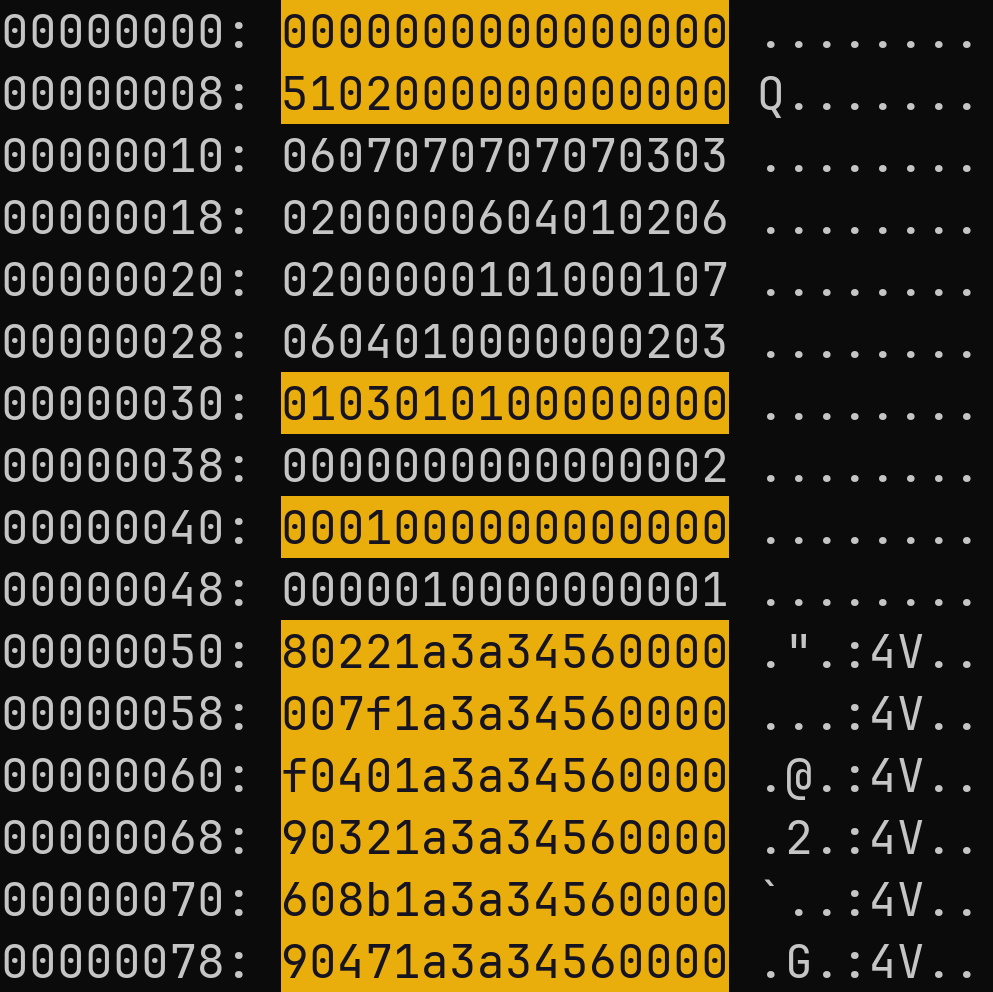
\includegraphics[width=16cm]{dataset/pointer_examples_1010-1644391327-heap_potential_pointer_highlight.png}
        \caption{Binary RAW heap dump file loaded using \texttt{vim} and \texttt{xxd}, from \textit{/Training/Training/scp/V\_7\_8\_P1/16/1010-1644391327-heap.raw}, with highlight on rows with 12 hexadecimal digits followed by 4 zeros.}
    \end{figure}

    We have information about the starting address of the heap using \lstinline[style=json]!"HEAP_START": "56343a198000"!. Considering that the example heap dump file contains $ 135169 $ bytes, this means that for this given heap dump file, the pointer addresses range from value $ 94782313037824_{10} $ and $ 94782313172993_{10} $. Note that the little-endian hexadecimal representation of the heap end address is \lstinline[language=c]!0x01901b3a3456! which is 12 character long, or 6 bytes long.

    Note that conversions here can get confusing, since potential pointer strings extracted from the heap dump file are given in little-endian hexadecimal format, but the heap start address from the JSON annotation file is given in big-endian hexadecimal format.

    \begin{minipage}{\dimexpr\linewidth-20pt}
        That way, we can refine the detection of potential pointers by only considering the bytes that are in the range of the heap. Potential pointers are highlighted with "<<<" in the following hex dump:

        \begin{lstlisting}[language=python, caption={Conversions function from hex strings to decimal $ int $ values}.]
        # conversion from hex to decimal
        def hex_str_to_int(hex_str: str) -> int:
            """
            Convert a normal (big-endian) hex string to an int.
            WARNING: HEAP_START in JSON is big-endian.
            """
            bytes_from_str = bytes.fromhex(hex_str)
            return int.from_bytes(
                bytes_from_str, byteorder='big', signed=False
            )
        
        def pointer_str_to_int(hex_str: str) -> int:
            """
            Convert a pointer hex string to an int.
            WARNING: Pointer hex strings are little-endian.
            """
            bytes_from_str = bytes.fromhex(hex_str)
            return int.from_bytes(
                bytes_from_str, byteorder='little', signed=False
            )
        \end{lstlisting}
    \end{minipage}

    Using the functions above, we can check which potential pointers are indeed within the heap dump range.

    \begin{minipage}{\dimexpr\linewidth-20pt}
        That way, we can refine the detection of potential pointers. In the following, pointers are highlighted with \lstinline[style=hexdump]!<<<! in the following hex dump:

        \begin{lstlisting}[style=hexdump, caption={8 bytes per line visualization of a Hex Dump from \textit{Training/basic/V\_7\_8\_P1/16/5070-1643978841-heap.raw}}]
            00000000: 0000000000000000 ........
            00000008: 5102000000000000 Q.......
            00000010: 0607070707070303 ........
            00000018: 0200000604010206 ........
            00000020: 0200000101000107 ........
            00000028: 0604010000000203 ........
            00000030: 0103010100000000 ........
            00000038: 0000000000000002 ........
            00000040: 0001000000000000 ........
            00000048: 0000010000000001 ........
            00000050: 80221a3a34560000 .".:4V.. <<<
            00000058: 007f1a3a34560000 ...:4V.. 
            00000060: f0401a3a34560000 .@.:4V.. <<<
            00000068: 90321a3a34560000 .2.:4V.. <<<
            00000070: 608b1a3a34560000 `..:4V.. <<<
            00000078: 90471a3a34560000 .G.:4V.. <<<
        \end{lstlisting}
    \end{minipage}

    \begin{minipage}{\dimexpr\linewidth-20pt}
        One last check we can do, is verify if the potential pointers are  8-bytes aligned. This can be done by checking if the last 3 bits of the potential address are 0, or using a modulo 8 operation. A simple python function can be used to check that:

        \begin{lstlisting}[language=python, caption={Python function to check if a potential pointer is 8-bytes aligned}]
            def is_pointer_aligned(pointer: int) -> bool:
                """
                Check if a pointer is 8-bytes aligned.
                """
                return pointer % 8 == 0
        \end{lstlisting}
    \end{minipage}

    Using this function on the potential pointers we have found so far, we can see that all of them are indeed 8-bytes aligned. This is a good sign for pointer detection, as we now have a range of tests that can be used to detect potential pointers from other potentially random values.

    Here is the pseudocode for the pointer detection algorithm. This algorithm is presented for a full heap dump file:

    \begin{algorithm}
        \caption{Pointer Detection Algorithm}
        \begin{algorithmic}[1]
        \Procedure{PointerDetection}{$\text{heapDumpFile, HEAP\_START}$}
            \State $\text{heapStart} \gets \text{hex\_str\_to\_int}(HEAP\_START)$
            \State $\text{heapEnd} \gets \text{heapStart} + \text{FileSize}(\text{heapDumpFile})$
            \State $\text{position} \gets 0$
            \State $\text{potentialPointers} \gets []$
            \While{$\text{position} < \text{FileSize}(\text{heapDumpFile})$}
                \State $\text{block} \gets \text{Read8Bytes}(\text{heapDumpFile, position})$
                \If{$\text{block} \neq 0$}
                    \State $\text{pointer} \gets \text{pointer\_str\_to\_int}(\text{block})$
                    \If{$\text{heapStart} \leq \text{pointer} \leq \text{heapEnd}$}
                        \If{$\text{is\_pointer\_aligned}(\text{pointer})$}
                            \State $\text{Append}(\text{pointer}, \text{potentialPointers})$
                        \EndIf
                    \EndIf
                \EndIf
                \State $\text{position} \gets \text{position} + 8$
            \EndWhile
            \State \Return $\text{potentialPointers}$
        \EndProcedure
        \end{algorithmic}
    \end{algorithm}

    This pseudocode outlines the steps for detecting potential pointers in the heap dump file. It starts by reading the heap dump file 8 bytes at a time. For each 8-byte block, it checks if the block is non-zero and within the heap range. If so, it checks if the potential pointer is 8-bytes aligned using the \texttt{is\_pointer\_aligned} function we described before. If all conditions are met, the potential pointer is added to the list of potential pointers. The algorithm returns this list at the end.
    
    \subsubsection{Detecting potential keys}
    % speak about SmartKex22 brute force approach
    % describe the algorithm to detect potential keys

    Encryption key prediction is the main focus of the present thesis. As such, we will now focus on how to detect potential keys in heap dump files. The paper \citetitle{SmartKex22} introduces 2 algorithms for key detection. The first one is a brute force approach that consists in trying all the possible keys in the heap dump file. The second one is a more sophisticated approach that uses a set of rules to detect potential keys.
    
    The first brute-force algorithm is given by:

    \begin{algorithm}[H]\label{alg:methods:dataset:smartkex22:brute_force}
    \caption{SSH keys brute-force algorithm from \citetitle{SmartKex22} \cite{SmartKex22}}
    \begin{algorithmic}[1]
    \Procedure{FindIVAndKey}{$\text{netPacket}, \text{heapDump}$}
        \State $\text{ivLen} \gets 16$ \Comment{Based on the encryption method}
        \State $\text{keyLen} \gets 24$ \Comment{Based on the encryption method}
        \State $i \gets \text{sizeof(cleanHeapDump)}$
        \State $r \gets 0$
        \While{$r < i$}
            \State $\text{pIV} \gets \text{heapDump}[r : r + \text{ivLen}]$
            \State $x \gets 0$
            \While{$x < i$}
                \State $\text{pKey} \gets \text{heapDump}[x : x + \text{keyLen}]$
                \State $f \gets \text{decrypt}(\text{netPacket}, \text{pIV}, \text{pKey})$
                \If{$f$ is TRUE}
                    \State \textbf{return} $\text{pIV}, \text{pKey}$
                \EndIf
                \State $x \gets x + 8$ \Comment{The IV is 8-bytes aligned}
            \EndWhile
            \State $r \gets x + 8$ \Comment{The key is 8-bytes aligned}
        \EndWhile
    \EndProcedure
    \end{algorithmic}
    \end{algorithm}
    
    This algorithm \ref{alg:methods:dataset:smartkex22:brute_force} outlines the brute-force approach for finding the Initialization Vector (IV) and the key. Initially, the lengths \(\text{ivLen}\) and \(\text{keyLen}\) are set based on the encryption method used for the heap. The algorithm then takes the first \(\text{ivLen}\) bytes from the heap dump to serve as the potential IV (\(pIV\)). Subsequently, \(\text{keyLen}\) bytes are extracted from the heap dump, starting from the first byte, to act as the potential key (\(pKey\)). The algorithm iterates through this potential key until it reaches the end of the heap dump. If decryption of the network packet is unsuccessful, the process is repeated by reading the next potential IV and the subsequent potential key \cite{SmartKex22}. 

    This algorithm is fairly straightforward, and can be implemented in a few lines of code. However, it is also very inefficient, as it tries all the possible keys in the heap dump file. It also needs some encrypted network packets to be able to test the keys, which are not included in the dataset. As such, we will not implement this algorithm.
    
    This is why the authors of the paper have also developed a more sophisticated algorithm that uses a set of rules to detect potential keys.

    No pseudocode is given for the second algorithm, but the paper \citetitle{SmartKex22} gives a description of the algorithm. It relies on the high-entropy assumption of encryption keys. The algorithm is inspired by image processing techniques, and can be described as follows:

    \begin{algorithm}
        \caption{Image-processing inspired Preprocessing Algorithm, as described in \citetitle{SmartKex22} \cite{SmartKex22}}
        \begin{algorithmic}[1]
        \Procedure{Preprocessing}{$\text{heapData}$}
            \State \textbf{Reshape} $\text{heapData}$ into $N \times 8$ matrix $X$
            \For{$i = 0$ to $N-1$}
                \For{$j = 0$ to $7$}
                    \State $Y[i][j] = |X[i][j] - X[i][j+1]| \& |X[i][j] - X[i+1][j]|$
                    \State $Z[i] = \text{count}(Y[i][k] == 0) \geq 4$
                    \If{$i < N-1$}
                        \State $R[i] = Z[i] \& Z[i+1]$
                    \EndIf
                \EndFor
            \EndFor
            \State \textbf{Extract} 128-byte slices from $R$ for training
        \EndProcedure
        \end{algorithmic}
    \end{algorithm}
    
    This Preprocessing Algorithm serves as a crucial step in adapting the heap data for machine learning models. The algorithm begins by reshaping the raw heap data into an \(N \times 8\) matrix \(X\), since keys are 8-bytes aligned \cite{SmartKex22}. Here, \(N \times 8\) is the size of the original heap data in bytes. It then calculates the discrete differences of the bytes in both vertical and horizontal directions, storing the results in matrix \(Y\). The algorithm employs a logical AND operation on these differences to identify high-entropy regions, which are likely candidates for encryption keys. Each 8-byte row in \(Y\) is examined for randomness, and if at least half of its bytes differ from adjacent bytes, it is marked as a potential part of an encryption key. The algorithm then filters out isolated rows that are unlikely to be part of an encryption key, resulting in an array \(R\). Finally, 128-byte slices are extracted from \(R\) for training the machine learning model. This preprocessing step not only adapts the data for machine learning but also narrows down the search space for potential encryption keys, thereby enhancing the efficiency of the subsequent steps. 

    However, this algorithm is not as efficient as it could be. It relies on using a kind of sliding window, which is not easily parallelizable. Also, the entropy-inspired computation is not as straightforward as it could be. That why we propose a new algorithm that is more efficient and more easily parallelizable.

    In order to perform some \acrshort{ml} techniques, and because the keys we are looking for can have a range of possible lengths (16, 24, 32, or 64 bytes), we shift the focus from detecting the full key, to just be able to predict the address of the key. That way, we can deal with keys of different sizes, and we can also use the same algorithm to detect the IV. This is why we will focus on detecting potential keys addresses, and not the full keys.

    We thus introduce a new algorithm for narrowing the search space for potential keys. This algorithm is inspired by the paper \citetitle{SmartKex22}, but is more efficient and more easily parallelizable, as it focuses on producing pairs of blocks of 8 bytes with high entropy. It uses directly the Shannon entropy formula, with each entropy computation being independent of the others.

    \begin{algorithm}
        \caption{Entropy Based Detection of Potential Key blocks}
        \begin{algorithmic}[1]
        \Procedure{EntropyDetection}{$\text{heapData}$}
            \State \textbf{Pad} $\text{heapData}$ with 0s to be 8-bytes aligned
            \State \textbf{Reshape} $\text{heapData}$ into $N \times 8$ matrix $X$
            \For{$i = 0$ to $N-1$,}
                \State $entropy[i] = \text{ShannonEntropy}(X[i])$ \Comment{Independents, compute in parallel.}
            \EndFor
            \State \textbf{Add} $entropy$ 2 by 2 pairs into $entropy\_pairs$ \Comment{Keep block indexes in resulting tuples.}
            \State \textbf{Sort} $entropy\_pairs$ by entropy as $sorted\_pairs$
            \State \Return $\text{SortedPairs}(\text{sorted\_pairs})$
        \EndProcedure
        \end{algorithmic}
    \end{algorithm}

    The \textit{Entropy Based Detection of Potential Key blocks} algorithm takes a raw heap dump, represented by the variable \texttt{heapData}, as input. The data is first padded with zeros to align it to 8-byte blocks and then reshaped into an $N \times 8$ matrix $X$. The Shannon entropy is computed for each 8-byte block in parallel, resulting in an array \texttt{entropy}. Subsequently, the entropy values of adjacent blocks are summed to form pairs, which are stored in \texttt{entropy\_pairs} along with their block indexes. These pairs are then sorted by their entropy sums to produce \texttt{sorted\_pairs}. The idea of using pairs of blocks instead of a single block or more than two blocks is related to the minimum key size, which is 16 bytes. This means that we need at least 2 blocks to be able to detect a potential key. The algorithm returns sorted pairs, so that we can easily extract the ones with the highest entropy sums. Given the index of a block, its actual memory address can be recomputed using the \texttt{HEAP\_START} address available in annotations.
    
    Using this algorithm, let's continue to explore our example heap dump file from \ref{lst:hexdump-8bytes}. We will use the following python function to compute the Shannon entropy of a given block of 8 bytes:

    \begin{minipage}{\dimexpr\linewidth-20pt}
    \begin{lstlisting}[language=python, caption={Python function to compute the Shannon entropy of a given block of 8 bytes}]
        def get_entropy(data: bytes):
            """
            Computes the entropy of a byte array, using Shannon's formula.
            """

            if len(data) == 0:
                return 0.0
            
            # Count the occurrences of each byte value
            _, counts = np.unique(data, return_counts=True)
            
            # Calculate the probabilities
            prob = counts / len(data)
            
            # Calculate the entropy using Shannon's formula
            entropy = -np.sum(prob * np.log2(prob))
            
            return entropy
    \end{lstlisting}
    \end{minipage}

    This function used NumPy array function for efficient computation. We can now use this function to compute the entropy of each block of 8 bytes in the heap dump file. We can then sort the pair of blocks by their entropy, and keep the ones with the highest entropy.
    
    When applied to the file \textit{Training/basic/V\_7\_8\_P1/16/5070-1643978841-heap.raw}, the algorithm produced $ 16896 $ entropy pairs, with $ 631 $ pairs having the maximum entropy sum. Another test using the index to address conversion and the JSON annotation file also indicate that all the 6 key addresses are within the $ 631 $ pairs with the highest entropy sum.
    
    This allows to reduce significantly the search space for potential keys, to already less that 4\% of the original heap dump file, which is significantly better that the 30\% reduction obtained by the preprocessing algorithm described in the paper SmartKex \cite{SmartKex22}, but less that the 2\% reduction obtained by the \acrshort{ml}-based processing algorithm described in the paper \cite{SmartKex22}. However, the same paper indicated that it was tested only for Key A and Key C, whereas this algorithm is tested for all the keys. Keep in mind that this is just an example for a single random file in the dataset, as a way to introduce the subject. In-depth experiments will be done in the dedicated chapter on \acrlong{ml}.

    Indeed, it is important to mention that we can rely on the JSON annotation files for providing labelling for key address prediction. Using this, we do not need to decrypt the network packets to be able to train our \acrshort{ml} models. This is a huge advantage, and is also required since we don't have the encrypted network packets in the dataset. Since we don't have those, and since the keys are already given, that is why we will focus on key address prediction, and not on key prediction.

    \subsection{Data structure exploration}
    Since the dataset contain whole heap dump file, we can also try to detect allocated chunks in those heap dumps. This can be done by looking for patterns in the heap dump file, in a similar fashion as we have done for potential pointers. However, for data structure, we can rely on our knowledge of the C library used to know exactly what to look for.
    
    Since OpenSSH is written in C, we can expect to find some C memory chunks in the heap dump files. C uses the \lstinline[language=c]|malloc| function to allocate memory. This function is used to allocate memory for a given data structure. It takes as input the size of the data structure to allocate, and returns a pointer to the allocated memory. We know that the dataset has been produced using \texttt{GLIBC 2.28} \ref{sec:methods:dataset:production_system_information}. Looking directly at the code for \lstinline[language=c]|malloc| in \texttt{GLIBC 2.28}, we can read in the comments that \say{Minimum overhead per allocated chunk: 4 or 8 bytes. Each malloc chunk has a hidden word of overhead holding size and status information} \cite{MallocGLIBC2001}. This is what we refer to as the \textit{malloc header}. This means that we can expect to find some 8-bytes aligned blocks in the heap dump file, that are not pointers, but that are the result of a \lstinline[language=c]|malloc| call. Detecting and using those \textit{malloc headers} is how we will try to detect memory chunks in heap dump files.

    In Linux on a \texttt{x86\_64} architecture, the malloc function typically uses a block (chunk) header to store metadata about each allocated block. This header is placed immediately before the block of memory returned to the user. The exact layout can vary depending on the implementation of the C library (e.g., glibc, musl), but generally, it contains the following:

    \begin{itemize}
        \item \textbf{Size of the Block}: The size of the allocated block, usually in bytes. This size often includes the size of the header itself and may be aligned to a multiple of 8 or 16 bytes.
        \item \textbf{Flags}: Various flags that indicate the status of the block, such as whether it is free or allocated, or whether the previous block is free or allocated. These flags are often stored in the least significant bits of the size field, taking advantage of the fact that the size is usually aligned, leaving the least significant bits zeroed.
    \end{itemize}

    \subsubsection{How \texttt{malloc} handles Heap Allocation}

    The \texttt{malloc} function in GLIBC 2.28 uses a boundary tag method to manage chunks of memory. Each chunk contains metadata that helps in the allocation and deallocation of memory \cite{MallocGLIBC2001} \cite{MallocInternalsWiki2023}. Below are the key components of a chunk:

    A chunk is a contiguous section of memory, in our case composed of several blocks of 8 bytes, that is handled by \texttt{malloc}. It contains the following components \cite{MallocInternalsWiki2023} \cite{StackExchangeMalloc2023}:

    \begin{enumerate}
        \item \textbf{Size of Previous Chunk}: This field exists only if the previous chunk is unallocated and its \texttt{P} (PREV\_INUSE) bit is clear. It helps in finding the front of the previous chunk.
        
        \item \textbf{Size of Chunk}: This field contains the size of the chunk in bytes along with three flags: \texttt{A} (NON\_MAIN\_ARENA), \texttt{M} (IS\_MMAPPED), and \texttt{P} (PREV\_INUSE). These flags are in the last 3 \acrshort{lsb}s of the size field. This precise block is considered in the following report as the \textit{malloc header} block. Note that the size of the chunk include the size of the \textit{malloc header}, chunk user data and \textit{footer} blocks.
        
        \item \textbf{User Data}: This is the actual memory space that is returned to the user.
        
        \item \textbf{Footer}: This is the same as the size of the chunk but is used for application data. Depending on how the chunk is represented, this is exactly the same as the \textbf{Size of Chunk} field. This is a more intuitive representation and is the one chosen in the schematic representation below.
        
        \item \textbf{Flags}:
        \begin{itemize}
            \item \texttt{A} (NON\_MAIN\_ARENA): Indicates if the chunk is in the main arena or a thread-specific arena.
            \item \texttt{M} (IS\_MMAPPED): Indicates if the chunk is allocated via \texttt{mmap}.
            \item \texttt{P} (PREV\_INUSE): Indicates if the previous chunk is in use. If false, it means the previous chunk is free.
        \end{itemize}
    \end{enumerate}

    The chunk allocation process involves the following concepts: 

    \begin{enumerate}
        \item \textbf{Initialization}: The very first chunk allocated always has the \texttt{P} bit set to prevent access to non-existent memory.
        
        \item \textbf{Free Chunks}: Free chunks are stored in circular doubly-linked lists. They contain forward and backward pointers to the next and previous chunks in the list.
        
        \item \textbf{Mmapped Chunks}: These chunks have the \texttt{M} bit set in their size fields and are allocated one-by-one.
        
        \item \textbf{Fastbins}: These are treated as allocated chunks and are consolidated only in bulk. These \textit{bins} are used to speed up the allocation process.
        
        \item \textbf{Top Chunk}: This is a special chunk that always exists. If it becomes less than \texttt{MINSIZE} bytes long, it is replenished.
    \end{enumerate}

    As explained directly in the code comments, an allocated chunk of 8 byte blocks can be described by the diagram below \cite{MallocGLIBC2001}. Note that is representation is personal to better suit the needs of our forensic analysis. The slight difference resides in the fact that the \texttt{footer} with the size of the considered chunk is represented as being part of the next chunk and not the current chunk. The footer of the previous chunk is actually the \texttt{mchunkptr} address. As stated in the GlicC wiki: \say{within the malloc library, a "chunk pointer" or \texttt{mchunkptr} does not point to the beginning of the chunk, but to the last word in the previous chunk - i.e. the first field in mchunkptr is not valid unless you know the previous chunk is free} \cite{MallocInternalsWiki2023}. Due to consideration of free/allocated chunks, it's actually easier to just consider the footer as being part of the next chunk, and not the current chunk. This is why the diagram below is slightly different from the one in the GLIBC wiki. This is just a difference in schematic representation, and does not change the actual data structure.

    \begin{figure}[H]
    \centering
    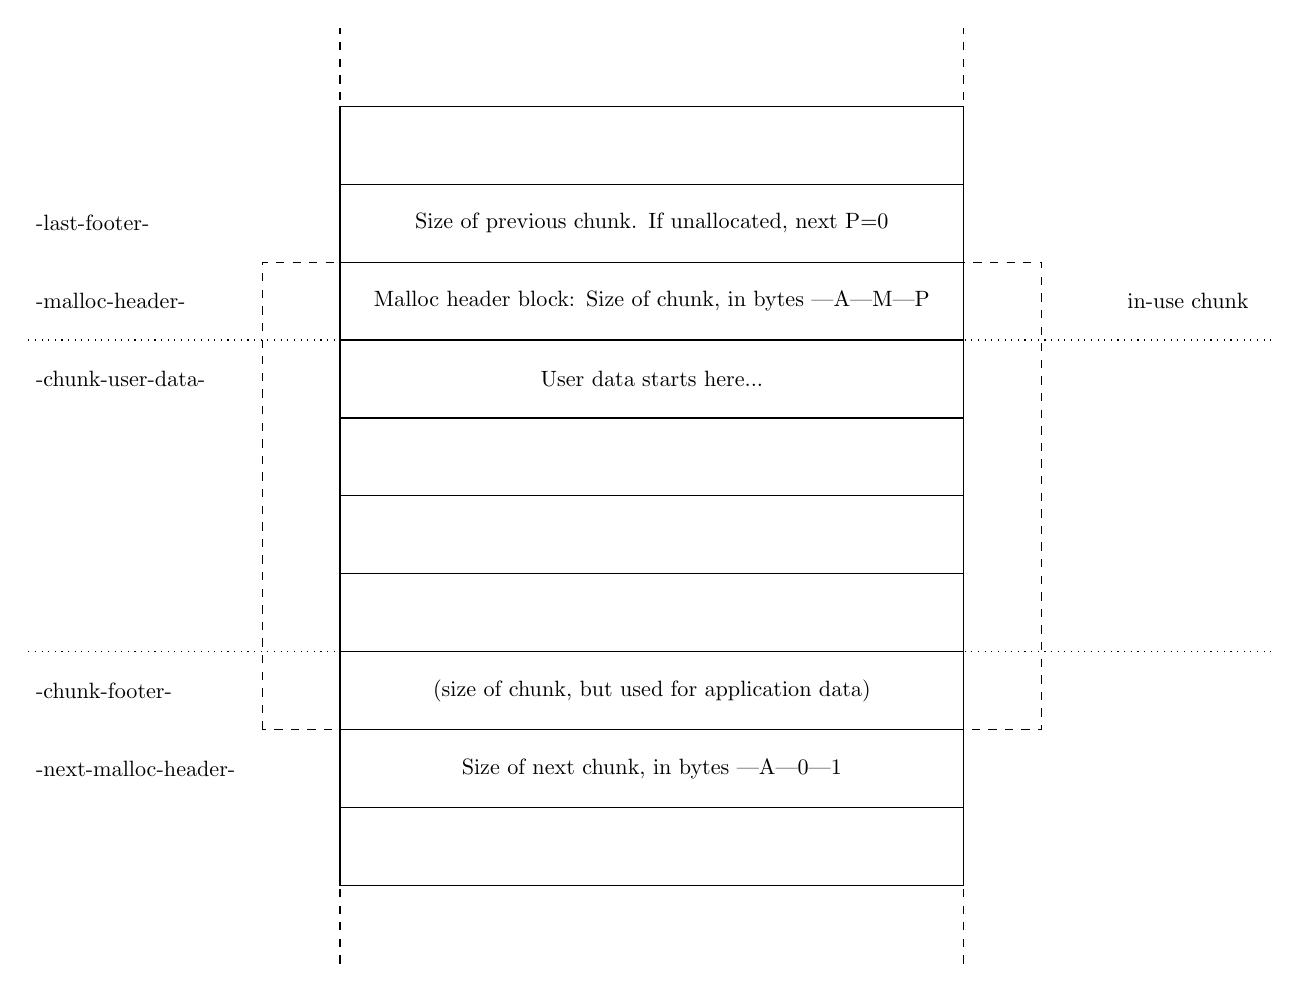
\begin{tikzpicture}[scale=0.99, every node/.style={scale=0.8}]
        % image from (0,0) to (16,12)
        
        % Draw rectangles
        \draw (4,1) rectangle (12,2);
        \draw (4,2) rectangle (12,3); % chunk-> Size of previous chunk
        \draw (4,3) rectangle (12,4); % malloc header (size of chunk)
        \draw (4,4) rectangle (12,5); %  mem-> user data starts here
        \draw (4,5) rectangle (12,6);
        \draw (4,6) rectangle (12,7);
        \draw (4,7) rectangle (12,8);
        \draw (4,8) rectangle (12,9); % nextchunk-> (app size of chunk)
        \draw (4,9) rectangle (12,10); % Size of next chunk
        \draw (4,10) rectangle (12,11);

        \draw[dashed] (3,3) rectangle (13,9);
        
        % after the rectangle step, the coordinates of the y axis are reversed ???
        % Dotted lines for user data
        \draw[dotted] (0,8) -- (16,8);
        \draw[dotted] (0,4) -- (16,4);

        % Dotted lines for memory band of 8 byte blocks
        \draw[dashed] (4,0) -- (4,12);
        \draw[dashed] (12,0) -- (12,12);
        
        % Labels
        \node[anchor=west] at (0,9.5) {-last-footer-};
        \node[anchor=west] at (0,8.5) {-malloc-header-};
        \node[anchor=west] at (0,7.5) {-chunk-user-data-};
        \node[anchor=west] at (0,3.5) {-chunk-footer-};
        \node[anchor=west] at (0,2.5) {-next-malloc-header-};

        \node[anchor=west] at (14,8.5) {in-use chunk};
        
        % Text inside rectangles
        \node[text width=14cm, align=center] at (8,9.5) {Size of previous chunk. If unallocated, next P=0};
        \node[text width=14cm, align=center] at (8,8.5) {Malloc header block: Size of chunk, in bytes |A|M|P};
        \node[text width=14cm, align=center] at (8,7.5) {User data starts here...};
        \node[text width=14cm, align=center] at (8,3.5) {(size of chunk, but used for application data)};
        \node[text width=14cm, align=center] at (8,2.5) {Size of next chunk, in bytes |A|0|1};
    \end{tikzpicture}
    \caption{Diagram of an allocated chunk in GLIBC 2.28 \cite{MallocGLIBC2001}.}
    \label{fig:allocated_chunk}
    \end{figure}

    The \texttt{malloc} function in GLIBC 2.28 uses a boundary tag method to manage chunks of memory. Each chunk contains metadata that helps in the allocation and deallocation of memory \cite{MallocGLIBC2001} \cite{MallocInternalsWiki2023}. The library stores available free chunks in circular doubly-linked lists called \say{bins}. This allows to quickly find a free chunk of memory of a given size. The problem is that we don't have access to those bins in the heap dump file. So to detect if a given chunk is in-use or free, we can rely on several methods. The first one is to look at the \texttt{P} bit of the malloc header. If it is set to 1, it means that the chunk is in use. If it is set to 0, it means that the chunk is free. 

    I also remarked that sometimes, the given heap dump file is cropped, and the last block is only composed of zeros and not complete. This is for instance the case with the last chunk of \textit{Training/basic/V\_7\_1\_P1/24/17016-1643962152-heap.raw}.

\begin{lstlisting}[language=bash, caption={Logs from chunk exploration script, related to the last chunk of the file \textit{Training/basic/V\_7\_1\_P1/24/17016-1643962152-heap.raw}. }]
WARN: Chunk [94022266975200] Chunk(block_index=10876, size=48176, flags=[A=False, M=False, P=True]) is out of bounds. Last block index: 16895 Iteration index: 16896 
WARN: Chunk [94022266975200] Chunk(block_index=10876, size=48176, flags=[A=False, M=False, P=True]) is out of bounds. Last block index: 16895 Iteration index: 16897
Chunk(block_index=10876, size=48176) is only composed of zeros.
\end{lstlisting}

    A free chunk contains the pointers of the next and previous free chunks in the heap, for its given bin. A representation of a free chunk, based directly on the code documentation \cite{MallocGLIBC2001}, is given below:

    \begin{figure}[H]
        \centering
        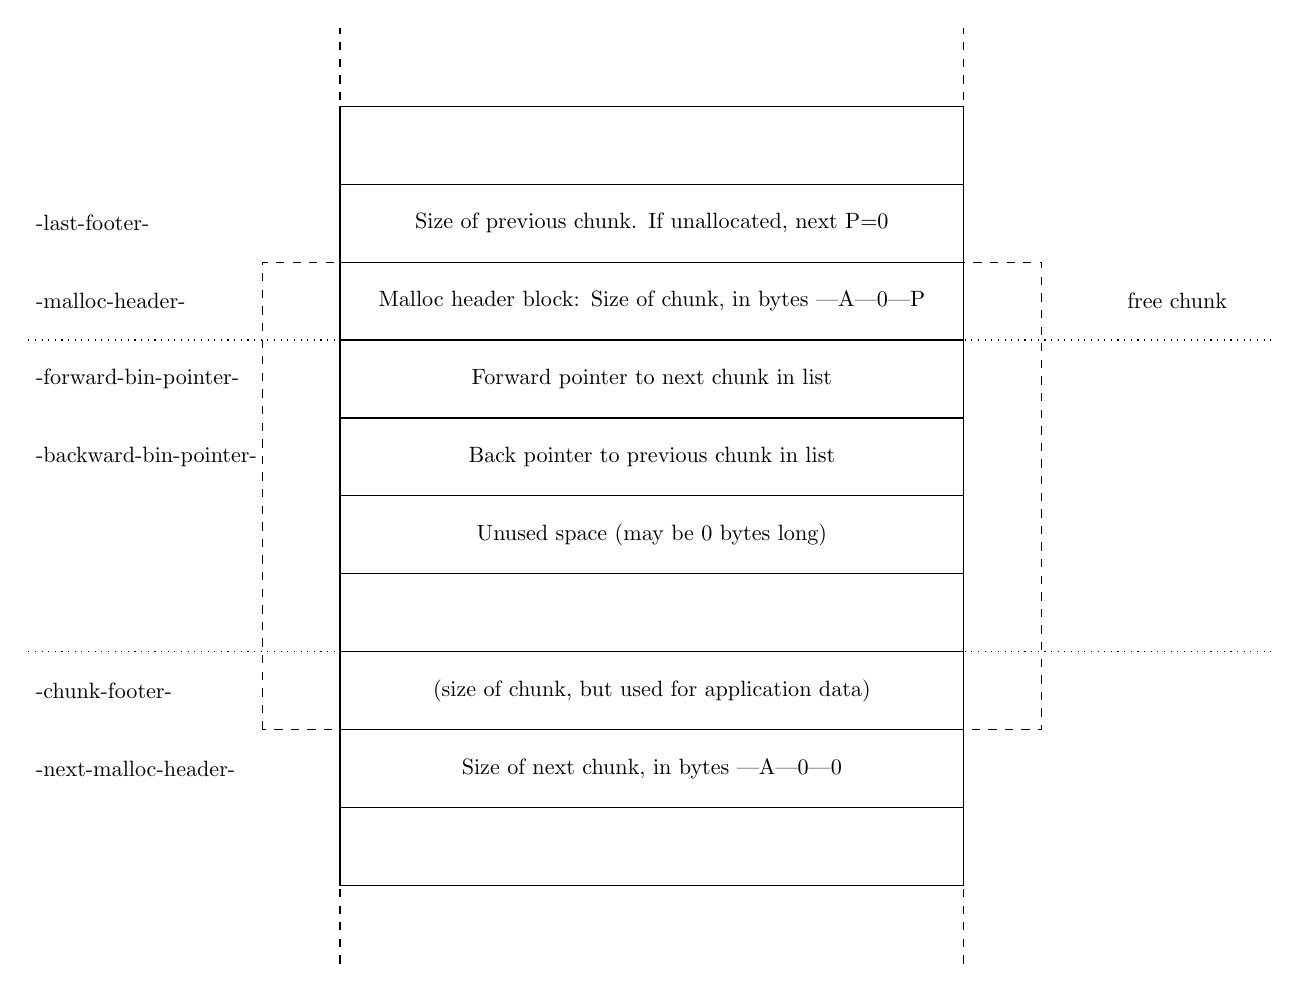
\begin{tikzpicture}[scale=0.99, every node/.style={scale=0.8}]
            % image from (0,0) to (16,12)
            
            % Draw rectangles
            \draw (4,1) rectangle (12,2);
            \draw (4,2) rectangle (12,3); % chunk-> Size of previous chunk
            \draw (4,3) rectangle (12,4); % malloc header (size of chunk)
            \draw (4,4) rectangle (12,5); %  mem-> user data starts here
            \draw (4,5) rectangle (12,6);
            \draw (4,6) rectangle (12,7);
            \draw (4,7) rectangle (12,8);
            \draw (4,8) rectangle (12,9); % nextchunk-> (app size of chunk)
            \draw (4,9) rectangle (12,10); % Size of next chunk
            \draw (4,10) rectangle (12,11);
    
            \draw[dashed] (3,3) rectangle (13,9);
            
            % after the rectangle step, the coordinates of the y axis are reversed ???
            % Dotted lines for user data
            \draw[dotted] (0,8) -- (16,8);
            \draw[dotted] (0,4) -- (16,4);
    
            % Dotted lines for memory band of 8 byte blocks
            \draw[dashed] (4,0) -- (4,12);
            \draw[dashed] (12,0) -- (12,12);
            
            % Labels
            \node[anchor=west] at (0,9.5) {-last-footer-};
            \node[anchor=west] at (0,8.5) {-malloc-header-};
            \node[anchor=west] at (0,3.5) {-chunk-footer-};
            \node[anchor=west] at (0,2.5) {-next-malloc-header-};

            \node[anchor=west] at (0,7.5) {-forward-bin-pointer-};
            \node[anchor=west] at (0,6.5) {-backward-bin-pointer-};
    
            \node[anchor=west] at (14,8.5) {free chunk};
            
            % Text inside rectangles
            \node[text width=14cm, align=center] at (8,9.5) {Size of previous chunk. If unallocated, next P=0};
            \node[text width=14cm, align=center] at (8,8.5) {Malloc header block: Size of chunk, in bytes |A|0|P};
            \node[text width=14cm, align=center] at (8,7.5) {Forward pointer to next chunk in list};
            \node[text width=14cm, align=center] at (8,6.5) {Back pointer to previous chunk in list};
            \node[text width=14cm, align=center] at (8,5.5) {Unused space (may be 0 bytes long)};
            \node[text width=14cm, align=center] at (8,3.5) {(size of chunk, but used for application data)};
            \node[text width=14cm, align=center] at (8,2.5) {Size of next chunk, in bytes |A|0|0};
        \end{tikzpicture}
        \caption{Diagram of a free chunk in GLIBC 2.28 \cite{MallocGLIBC2001}.}
        \label{fig:free_chunk}
    \end{figure}

    \subsubsection{Chunk chaining}
    The chunk chaining algorithm relies on the \textbf{chunk chaining assumption} \ref{sec:methods:dataset:assumptions}. This assumption states that the allocator allocates chunks after chunks, and that the chunks are contiguous in memory. This means that we can expect to find the malloc header of the next chunk at the address $ \text{current\_malloc\_header\_chunk\_address} + \text{current\_chunk\_size} + 8 $, where 8 is the size of the malloc header block, or $ \text{current\_chunk\_user\_data\_address} + \text{current\_chunk\_size} $. It is the case for both free and allocated chunks. This is why we can use this assumption to detect chunks in the heap dump file. 
    
    This necessitates to understand malloc header blocks, and how they are represented in the heap dump file. In the specific case of \texttt{GLIBC 2.28}, the malloc header is defined as follows:

    \begin{minipage}{\dimexpr\linewidth-20pt}
        \begin{lstlisting}[language=c, caption={Malloc header definition in \texttt{GLIBC 2.28}}]
            #define SIZE_BITS (PREV_INUSE | IS_MMAPPED | NON_MAIN_ARENA)
        \end{lstlisting}
    \end{minipage}
    
    Since the malloc header respects the endianness of the system, we can expect to find the malloc header in little-endian format in the heap dump file. Using vim on \textit{Training/basic/V\_7\_8\_P1/16/5070-1643978841-heap.raw}, we can use the following command to find some potential malloc headers:

    \begin{lstlisting}[language=bash, caption={Vim command to find potential malloc headers}]
        :/[0-9a-f]\{4}0\{12}
    \end{lstlisting}
    
    This gives something like the following:

    \begin{figure}[H]
        \centering
        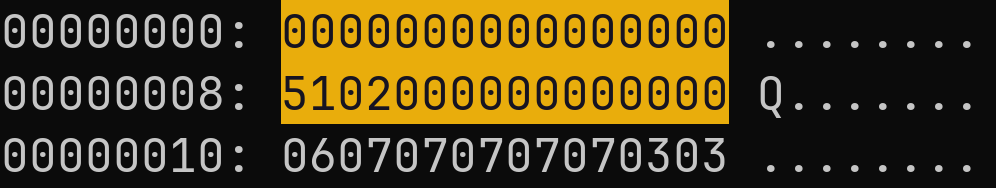
\includegraphics[width=16cm]{dataset/structure_examples_1010-1644391327-heap_potential_malloc_header_highlight_heap_start.png}
        \caption{Attempt at malloc header detection in \textit{Training/basic/V\_7\_8\_P1/16/5070-1643978841-heap.raw}, at heap start.}
    \end{figure}

    Indeed, after a first zero block of 8 bytes (potential previous chunk footer), we expect a first data structure to be allocated at the start of the heap. Here this data structure is of size $ 5102000000000000_{16LE} $ (little-endian hex format) or $ 593_{10} $ bytes. The fact that it is an odd number is due to the \acrshort{lsb} being set to 1, to indicate that the preceding chunk is allocated (P flag). This means that the real size of the structure is actually $ 593_{10} - 1_{10} = 592_{10} $. This value is 8-byte aligned.

    Since we know that the allocator allocates chunks after chunks, we can expect the next chunk to be allocated at the address $ 5102000000000000_{16LE} + 592_{10} + 8_{10} = 5882193a34560000_{16LE} =  $. Note that we need to add 8 to the size to account for the malloc header block.
    
    In vim, since the address start at 0, we have to look at $ 592_{10} + 8_{10} = 258_{16} $. Let's have a look there:

    \begin{figure}[H]
        \centering
        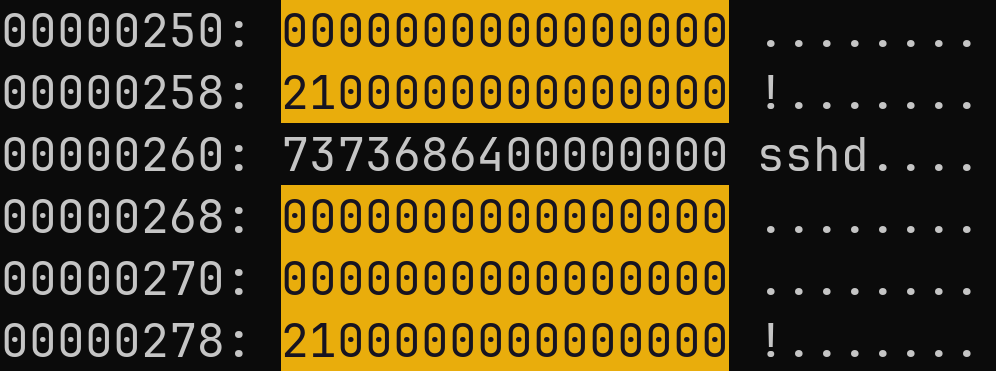
\includegraphics[width=16cm]{dataset/structure_examples_1010-1644391327-heap_potential_malloc_header_highlight_0x250.png}
        \caption{Attempt at malloc header detection in \textit{Training/basic/V\_7\_8\_P1/16/5070-1643978841-heap.raw}, at index $ 592_{10} = 250_{16} $.}
    \end{figure}

    There, we can see a zero block, followed by what we can expect to be another malloc header at address $ 258_{16} $. By doing the same process, we can thus propose an algorithm to detect the malloc headers, and thus the structures in the heap dump file.

    First, here is a simple algorithm to extract all the necessary information from a malloc header block:

    \begin{algorithm}[H]\label{alg:malloc_header_parsing}
        \caption{Malloc Header Parsing Algorithm}
        \begin{algorithmic}[1]
            \Procedure{MallocHeaderParsing}{$block$}
            \Require $block$ is a block of 8 bytes
            \Ensure $MallocHeader$ object
            \Ensure $Flags$ object
            \State \textbf{Note:} In this algorithm, $\&$ represents bitwise AND, and $\sim$ represents bitwise negation.
            \State $size\_and\_flags \leftarrow \text{ConvertBytesToInteger}(block, \text{'little-endian'})$
            \State $size \leftarrow size\_and\_flags \; \& \; (\sim 0x07)$ \Comment{Clear the last 3 bits to get the size}
            \State $Flags.a \leftarrow \text{bool}(size\_and\_flags \; \& \; 0x04)$
            \State $Flags.m \leftarrow \text{bool}(size\_and\_flags \; \& \; 0x02)$
            \State $Flags.p \leftarrow \text{bool}(size\_and\_flags \; \& \; 0x01)$
            \State \Return $MallocHeader\{size, Flags\}$
        \EndProcedure
        \end{algorithmic}
    \end{algorithm}

    We can also isolate the size parsing algorithm into a handy function:

    \begin{algorithm}[H]\label{alg:convert_to_size}
        \caption{Malloc Header block to size conversion Algorithm}
        \begin{algorithmic}[1]
            \Procedure{ConvertToSize}{$block$}
            \Require $block$ is a block of 8 bytes
            \State \textbf{Note:} In this algorithm, $\&$ represents bitwise AND, and $\sim$ represents bitwise negation.
            \State $size\_and\_flags \leftarrow \text{ConvertBytesToInteger}(block, \text{'little-endian'})$
            \State $size \leftarrow size\_and\_flags \; \& \; (\sim 0x07)$ \Comment{Clear the last 3 bits to get the size}
            \State \Return $size$
        \EndProcedure
        \end{algorithmic}
    \end{algorithm}

    Based on those algorithms, and in a similar fashion as what we have done manually by exploring the heap dump file with vim, we can propose the following algorithm to detect the malloc headers in a heap dump file:

    \begin{algorithm}[H]\label{alg:malloc_header_chaining}
        \caption{Malloc Header Chaining Algorithm}
        \begin{algorithmic}[1]
        \Procedure{MallocHeaderDetection}{$heapDumpFile$}
            \State \textbf{Note:} ConvertToSize is equivalent to MallocHeaderParsing($block$).size \Comment{See \ref{alg:convert_to_size}}
            \State \textbf{Initialize} malloc\_header\_list to empty list
            \State $position \gets 0$
            \While{$position < \text{FileSize}(heapDumpFile)$}
                \State $block \gets \text{Read8Bytes}(heapDumpFile, position)$
                \If{$\text{block} \neq 0$}
                    \State $size \gets \text{ConvertToSize}(block)$ \Comment{Be careful with flags}
                    \State \textbf{Assert} $size != 0$
                    \State \textbf{Assert} $size \mod 8 = 0$ \Comment{Check if the size is 8-bytes aligned}
                    \State $position \gets position + size$ \Comment{Leap over data structure.}
                \Else
                    \State $position \gets position + 8$
                \EndIf
            \EndWhile
            \State \Return $malloc\_header\_list$
        \EndProcedure
        \end{algorithmic}
    \end{algorithm}

    The idea behind the malloc header detection algorithm is simple. We start at the beginning of the heap dump file, and we look for the first non-zero block. Then we assume that the next block is a malloc header. We convert it to a size, and then leap over the user data and the footer up to the next chunk malloc header block index. The process is repeated until reaching the end of the heap dump file.

    Note that in case of a problem, like when the size obtained from malloc header parsing is equal to 0, this means that the heap dump chaining is broken. This has been handled in the dataset cleaning section \ref{sec:methods:dataset:cleaning}. 

    \subsubsection{Chunk chaining example}
    The program \texttt{chunk\_algorithms.py} has been developed specifically to test the chunk parsing and refine the associated algorithms.

    We can test our chunk parsing algorithm on a test file in the cleaned dataset.

    \begin{lstlisting}[language=bash, caption={Testing chunk parsing on \textit{Training/basic/V\_7\_1\_P1/24/17016-1643962152-heap.raw}. Partial log output. }]
$ python src/data_structure_detection.py --input /home/onyr/code/phdtrack/phdtrack_data_clean/Training/Training/basic/V_7_1_P1/24/17016-1643962152-heap.raw --debug
    Datetime: 2023_09_27_17_08_23_157209
    Chunk [1]: Chunk(block_index=2, size=592, flags=[A=False, M=False, P=True])
    Chunk [2]: Chunk(block_index=76, size=32, flags=[A=False, M=False, P=True])
    Chunk [3]: Chunk(block_index=80, size=32, flags=[A=False, M=False, P=True])
    Chunk [4]: Chunk(block_index=84, size=32, flags=[A=False, M=False, P=True])
    Chunk [5]: Chunk(block_index=88, size=32, flags=[A=False, M=False, P=True])
    Chunk [6]: Chunk(block_index=92, size=192, flags=[A=False, M=False, P=True])
    Chunk [7]: Chunk(block_index=116, size=32, flags=[A=False, M=False, P=True])
    Chunk [8]: Chunk(block_index=120, size=32, flags=[A=False, M=False, P=True])
    Chunk [...]: ...
    Chunk [911]: Chunk(block_index=10194, size=128, flags=[A=False, M=False, P=True])
    Chunk [912]: Chunk(block_index=10210, size=256, flags=[A=False, M=False, P=True])
    Chunk [913]: Chunk(block_index=10242, size=160, flags=[A=False, M=False, P=True])
    Chunk [914]: Chunk(block_index=10262, size=512, flags=[A=False, M=False, P=True])
    Chunk [915]: Chunk(block_index=10326, size=1296, flags=[A=False, M=False, P=True])
    Chunk [916]: Chunk(block_index=10488, size=1552, flags=[A=False, M=False, P=True])
    Chunk [917]: Chunk(block_index=10682, size=1552, flags=[A=False, M=False, P=True])
    Chunk [918]: Chunk(block_index=10876, size=48176, flags=[A=False, M=False, P=True])
    -----------> Statistics:
    Total number of files: 1
    Total number of chunks: 918
    Total number of blocks: 16896
    Total number of chunks with P=1: 903
    Total number of chunks with M=1: 0
    Total number of chunks with A=1: 0
    Total number of chunks only composed of zeros: 1
    \end{lstlisting}

    Looking at the first allocated chunks, we recognize what we had seen manually with vim for the file \textit{Training/basic/V\_7\_8\_P1/16/5070-1643978841-heap.raw}. The first chunk is of size 592, and the next one is of size 32. This is exactly what we had seen manually. It is a good sign that our algorithm is working as expected. We can also see that the last chunk is of size 48176, which is significantly bigger than the other chunks. This chunk is only composed of zeros, and is truncated, meaning that its size if bigger than the actual size of the heap dump file. 
    
    \subsubsection{Distinguishing between free and allocated chunks}
    The malloc header chaining algorithm allows to detect memory chunks in the heap dump file. However, it does not allow to distinguish between free and allocated chunks. This is a problem, since we want to be able to distinguish between free and allocated chunks, to be able to detect potential data structures and filter out useless blocks.
    
    Considering the structural differences between a free and in-use block, it's possible to try distinguishing free blocks by their \textit{forward} and \textit{backward} pointers. The issue is that the head dump raw file are not provided with any \textit{bins} information. As such, distinguishing between two normal pointers and the ones expected inside a free block is a non-trivial task. Hence, the tests performed on this idea are inconclusive. A more straightforward technique is to rely on the \texttt{P} malloc header flags. 
    
    \begin{figure}[H]
        \centering
        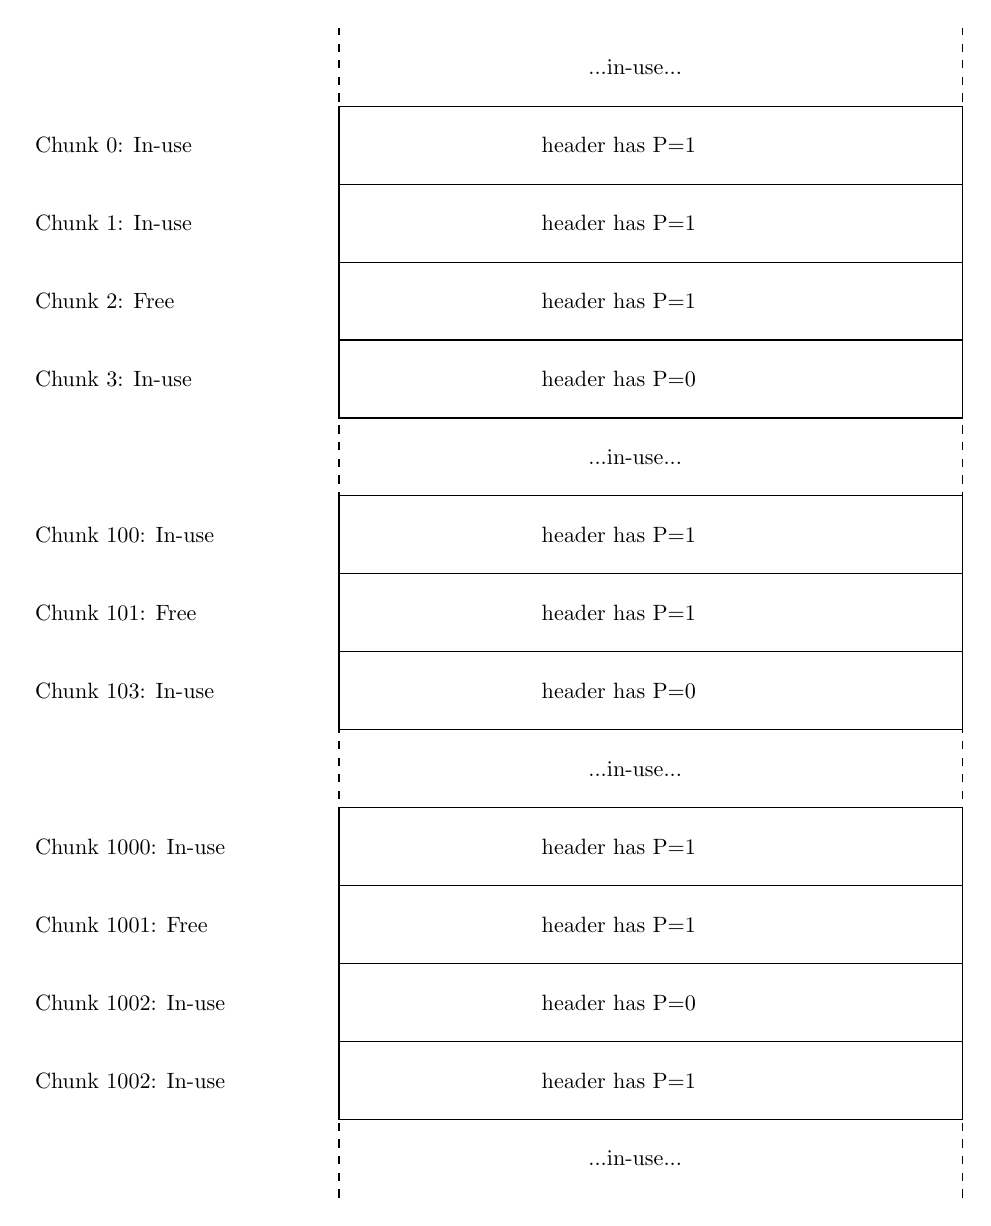
\begin{tikzpicture}[scale=0.99, every node/.style={scale=0.8}]
            % Dotted lines for memory band of 8 byte blocks
            \draw[dashed] (4,0) -- (4,15);
            \draw[dashed] (12,0) -- (12,15);

            % ... Ellipses to represent continuation
            \node[anchor=east] at (8.5,14.5) {...in-use...};

            % Chunk - In-use
            \draw (4,13) rectangle (12,14);
            \node[anchor=west] at (0,13.5) {Chunk 0: In-use};
            \node[anchor=west] at (6.5,13.5) {header has P=1};

            % Chunk - In-use
            \draw (4,12) rectangle (12,13);
            \node[anchor=west] at (0,12.5) {Chunk 1: In-use};
            \node[anchor=west] at (6.5,12.5) {header has P=1};
            
            % Chunk - Free
            \draw (4,11) rectangle (12,12);
            \node[anchor=west] at (0,11.5) {Chunk 2: Free};
            \node[anchor=west] at (6.5,11.5) {header has P=1};

            % Chunk - In-use
            \draw (4,10) rectangle (12,11);
            \node[anchor=west] at (0,10.5) {Chunk 3: In-use};
            \node[anchor=west] at (6.5,10.5) {header has P=0};
    
            % Chunks - from top to bottom (inverted order)
            % ... Ellipses to represent continuation
            \node[anchor=east] at (8.5,9.5) {...in-use...};

            % Chunk - In-use
            \draw (4,8) rectangle (12,9);
            \node[anchor=west] at (0,8.5) {Chunk 100: In-use};
            \node[anchor=west] at (6.5,8.5) {header has P=1};
            
            % Chunk - Free
            \draw (4,7) rectangle (12,8);
            \node[anchor=west] at (0,7.5) {Chunk 101: Free};
            \node[anchor=west] at (6.5,7.5) {header has P=1};
            
            % Chunk - In-use, P=0
            \draw (4,6) rectangle (12,7);
            \node[anchor=west] at (0,6.5) {Chunk 103: In-use};
            \node[anchor=west] at (6.5,6.5) {header has P=0};
            
            % ... Ellipses to represent continuation
            \node[anchor=east] at (8.5,5.5) {...in-use...};
            
            % Chunk - In-use
            \draw (4,4) rectangle (12,5);
            \node[anchor=west] at (0,4.5) {Chunk 1000: In-use};
            \node[anchor=west] at (6.5,4.5) {header has P=1};
            
            % Chunk - Free
            \draw (4,3) rectangle (12,4);
            \node[anchor=west] at (0,3.5) {Chunk 1001: Free};
            \node[anchor=west] at (6.5,3.5) {header has P=1};
            
            % Chunk - In-use, P=0
            \draw (4,2) rectangle (12,3);
            \node[anchor=west] at (0,2.5) {Chunk 1002: In-use};
            \node[anchor=west] at (6.5,2.5) {header has P=0};

            % Chunk - In-use,
            \draw (4,1) rectangle (12,2);
            \node[anchor=west] at (0,1.5) {Chunk 1002: In-use};
            \node[anchor=west] at (6.5,1.5) {header has P=1};
            
            % ... Ellipses to represent continuation
            \node[anchor=east] at (8.5,0.5) {...in-use...};
    
        \end{tikzpicture}
        \caption{Heap dump showing a mix of free and in-use chunks. Note: each chunk immediately after a free chunk has a P flag set to 0. Each rectangle represents a chunk.}
        \label{fig:heap_dump}
    \end{figure}
    
    For a given chunk, the follow-up chunk in ascending address number, contains such a flag in its header block. If the flag value is 0, then the current chunk is free. If the flag value is 1, then the current chunk is in use by the program. This is the technique that has been used in the final implementation of the chunk chaining algorithm. 

    \begin{algorithm}[H]
        \caption{Chunk Parsing Algorithm}
        \begin{algorithmic}[1]
        \Procedure{ChunkParsing}{$heapDumpFile, HEAP\_START$}
            \State \textbf{Note:} ConvertToSize is equivalent to MallocHeaderParsing($block$).size
            \State \textbf{Note:} Get8BytesBlocks returns a list of 8 bytes blocks from the heap dump file.
            \Ensure $MallocHeader$ object
            \Ensure $Flags$ object
            \Ensure $Chunk$ object
            \Ensure $HEAP\_START$ provided from annotation file is a correct address.
            \State \textbf{Note:} In this algorithm, $\&$ represents bitwise AND, and $\sim$ represents bitwise negation.
            \State \textbf{Initialize} $chunk\_list$ to empty list
            \State $blocks \gets \text{Get8BytesBlocks}(heapDumpFile)$
            \State \textbf{Initialize} $index \gets 0$
            \While{$index < lenght(blocks)$}
                \State $block \gets blocks[index]$
                \State \textbf{Initialize} $Chunk$ to empty object
                \If{$\text{block} \neq 0$}
                    \State $Chunk.header : \{size, Flags\} \gets \text{MallocHeaderParsing}(block)$ \Comment{See \ref{alg:malloc_header_parsing}}
                    \State \textbf{Assert} $Chunk.header.size \geq 2 $ \Comment{Must contains at least header and footer}
                    \State \textbf{Assert} $Chunk.header.size \mod 8 = 0$ \Comment{Check if the size is 8-bytes aligned}
                    \State $Chunk.block\_index \gets index$ \Comment{Index of the first block of the chunk after header}
                    \State $Chunk.address \gets HEAP\_START + (index * 8)$ \Comment{Address of $block\_index$}
                    \State $footer\_index \gets index + Chunk.header.size - 1$ \Comment{Index of the footer block}
                    \If{$footer\_index < lenght(blocks)$}
                        \State $footer \gets blocks[footer\_index]$
                        \If{$\text{ConvertToSize}(footer) = Chunk.footer.size$}
                            \State $Chunk.correct_footer \gets True$
                        \Else
                            \State $Chunk.correct_footer \gets False$
                        \EndIf
                    \Else
                        \State $Chunk.correct_footer \gets False$
                    \EndIf
                    \State $next\_chunk\_header\_index \gets index + Chunk.header.size$ \Comment{Index of the next chunk header block}
                    \If{$next\_chunk\_header\_index < lenght(blocks)$}
                        \State $next\_chunk\_header \gets blocks[next\_chunk\_header\_index]$
                        \State $Chunk.is\_in\_use \gets \text{MallocHeaderParsing}(next\_chunk\_header).flags.p$
                    \Else
                        \State $Chunk.is\_in\_use \gets False$ \Comment{See \footnote{Experiments show that last chunk can be cropped and in that case, is only composed of zeros. We can thus consider it as free.}}
                    \EndIf
                    \State $index \gets index + Chunk.header.size$ \Comment{Leap over chunk.}
                \Else
                    \State $index \gets index + 8$ \Comment{Leap over zero block.}
                \EndIf
            \EndWhile
            \State \Return $malloc\_header\_list$
        \EndProcedure
        \end{algorithmic}
    \end{algorithm}

    Note that this algorithm is based on the malloc header chaining algorithm \ref{alg:malloc_header_chaining}. The main difference is that we now have access to the malloc header flags from the following chunk, and that we can thus distinguish between free and allocated chunks. The algorithm also includes the footer parsing technique discussed briefly in the following section.

    \subsubsection{Chunk footer}
    The documentation of the \texttt{malloc} function of GLIBC  states that the footer of a chunk is the same as the size of the chunk considered. In the current report, we represent the footer as being part of the chunk itself.

    Below are two chunks content of similar size:

    \begin{lstlisting}[language=bash, caption={Printing some free and in-use chunks from \textit{Training/basic/V\_7\_1\_P1/24/17016-1643962152-heap.raw}.}]
Printing Chunk [addr:0x80a2d1438355] [status:in-use] [footer:incorrect] Chunk(block_index=80, size=32, flags=[A=False, M=False, P=True])
        Block [79]: 	b'!\x00\x00\x00\x00\x00\x00\x00' 		33 		-malloc-header-
        Block [80]: 	b'\xa0\xa2\xd1C\x83U\x00\x00' 		94022266888864 		
        Block [81]: 	b'\xc0\xa2\xd1C\x83U\x00\x00' 		94022266888896 		
        Block [82]: 	b'\x00\x00\x00\x00\x00\x00\x00\x00' 		0 		-footer-
Printing Chunk [addr:0xa09fd2438355] [status:free] [footer:correct] Chunk(block_index=8180, size=32, flags=[A=False, M=False, P=True])
        Block [8179]: 	b'!\x00\x00\x00\x00\x00\x00\x00' 		33 		-malloc-header-
        Block [8180]: 	b'\xb0\xbc\xe1\xeeS\x7f\x00\x00' 		139998466784432 		
        Block [8181]: 	b'\xb0\xbc\xe1\xeeS\x7f\x00\x00' 		139998466784432 		
        Block [8182]: 	b' \x00\x00\x00\x00\x00\x00\x00' 		32 		-footer-
    \end{lstlisting}

    Here, the status of the chunk has been detected using the \texttt{P} flag technique. At first sight, those two blocks seems similar. The first 2 blocks in the user data space of the chunks both seems to contain what looks like pointers. As one can see, the first chunk in this example, with a \texttt{block\_index=80} has clearly a malloc header and footer as expected. Note that here, the value $33$ represents the size of the block ($32$ bytes which correspond to 4 blocks) with the \acrshort{lsb} being set to 1 meaning the preceding chunk is in use. However, the in-use block footer doesn't correspond to the value we expect. This difference of behavior is observed throughout the cleaned dataset. 

    \subsection{Discussing chunk parsing for problem scale reduction}
    Now that we have presented all the necessary knowledge and algorithms used to be able to parse the RAW heap dump files, we can discuss the results of those algorithms and their uses and limitations. Many tests have been needed in order to develop the final algorithms. This testing process has also unveiled some interesting properties of the dataset that will be used as basis for the semantic embedding of the memory graph representation and subsequent machine learning steps.

    The program \texttt{chunk\_algorithms.py} has been developed specifically to test the chunk parsing and refine the associated algorithms on the cleaned dataset. Below are presented the global statistics produced by the final version of the program:

    \begin{lstlisting}[language=bash, caption={Printing cleaned dataset chunk parsing global statistics.}]
        Input is directory: /home/onyr/code/phdtrack/phdtrack_data_clean/
        Found 26191 files in /home/onyr/code/phdtrack/phdtrack_data_clean/.
        Processing files: 100%|\blacksquare \blacksquare \blacksquare \blacksquare \blacksquare | 26191/26191 [12:11<00:00, 35.81it/s, file=7091-1650972335]
        ------> Statistics:
        Total number of parsed files: 26191
        Total number of skipped files: 0
        Total number of chunks: 37682063
        Total number of blocks: 674232832
        Total number of chunks with P=1: 37346373
        Total number of chunks with M=1: 0
        Total number of chunks with A=1: 0
        Total number of free chunks: 354410
        Total number of chunks only composed of zeros: 18720
        Total number of blocks in free chunks: 183331224
        Total number of chunks with correct footer value: 1009522
        Total number of chunks both free and with correct footer value: 335690
        Total number of chunks free and annotated: 0
        Total number of potential footers with annotations (should be 0): 0
        Total number of annotated chunks: 209528
        Total number of chunks in use, with correct footer, and annotated: 7668
        Total number of chunks in use, with correct footer, and key annotated: 7668
        Percentage of free chunks: 0.9405270619074121%
        Percentage of blocks in free chunks: 27.19108523033183%
        Percentage of free chunks with correct footer value: 94.71798199825061%
        Percentage of in-use chunks with correct footer value: 1.8051818044922352%
        Average number of annoted chunks per file: 8.0
        Average number of chunks in use with correct footer and annotated per file: 0.2927723263716544
        Set of sizes of key chunks: {32, 48, 64}
        Sizes of key chunks with their number of occurences:
        Size: 32  Number of occurences: 34366
        Size: 48  Number of occurences: 109346
        Size: 64  Number of occurences: 13434
        Number of sizes: 157146
        Number of unique sizes: {32, 48, 64}
    \end{lstlisting}

    The cleaned dataset contains 26191 RAW files and their corresponding annotation files. The program has been able to parse all those files, and has been able to detect 37682063 chunks, which represents 674232832 blocks. This is a huge number of blocks. The goal being to be able to predict which of those blocks are first key blocks, we need to be able to filter out the useless blocks as much as possible to both optimize computations and scale down the problem. 

    Using the \texttt{P} flag technique, we can see that 37346373 chunks are in use, and 354410 chunks are free. Although the proportion of free chunks is only 0.94\%, there are 27.19\% of the blocks that are in free chunks. More importantly, we can see that no free chunk is annotated. This means we can filter out all free chunks and their blocks. This allows a huge reduction of the scale of the problem. 
    
    The average number of annotated chunks per file being a perfect value of 8, this means that all the parsed files indeed contains the 6 key annotations with the additional \texttt{SSH\_STRUCT} and \texttt{SSH\_KEY} annotations. The dataset is very imbalanced since we have only 6 keys times the number of RAW files as positive labels and the rest as negative, thus the need for advanced reduction techniques. 

    \subsubsection{From a block-based to a chunk-based approach}
    
    The exact code to annotate the chunks can be as simple as the following:

    \begin{algorithm}[H]
        \caption{Annotate Chunk Algorithm}
        \begin{algorithmic}[1]
        \Procedure{AnnotateChunk}{$chunk, keys\_addresses, ssh\_struct\_addr, session\_state\_addr$}
            \Ensure $chunk$ object
            \Ensure $keys\_addresses$ list of integers
            \Ensure $ssh\_struct\_addr$ integer
            \Ensure $session\_state\_addr$ integer
            \State \textbf{Note:} Annotations should be done after free chunk detection.
            
            \Procedure{AssertChunkUsedThenAnnotate}{$chunk, annotation$}
                \State \textbf{Assert} $chunk.is\_in\_use$ \Comment{Make sure we don't annotate free chunks}
                \State $chunk.annotations.append(annotation)$
            \EndProcedure
            
            \If{$chunk.address \in keys\_addresses$}
                \State \textsc{AssertChunkUsedThenAnnotate}($chunk, ChunkAnnotation.ChunkContainsKey$)
            \ElsIf{$chunk.address = ssh\_struct\_addr$}
                \State \textsc{AssertChunkUsedThenAnnotate}($chunk, ChunkAnnotation.ChunkContainsSSHStruct$)
            \ElsIf{$chunk.address = session\_state\_addr$}
                \State \textsc{AssertChunkUsedThenAnnotate}($chunk, ChunkAnnotation.ChunkContainsSessionState$)
            \EndIf
        \EndProcedure
        \end{algorithmic}
    \end{algorithm}
    
    This algorithm in itself and the results observed is an important discovery. The annotations are actually always given for the \texttt{chunk.address} which corresponds to the address of the first block after the malloc header block. This means that the annotations are actually given for the beginning of the user data space of a chunk. This is crucial discovery, since it means that we can filter out the malloc header and footer blocks, and only keep the first block of the user data space of the chunks we want to embed. There are $674232832 - 183331224 = 490901608$ blocks in use. But there is only $37346373$ chunks in use. This means that we can reduce the number of blocks to embed from $490901608$ to $37346373$ which is an additional reduction applied after the previous filtering that reduces the scale of the problem by a factor of 13. 

    \subsubsection{Using chunk footer for filtering is not possible}
    
    Now let's look at the footer parsing. We can see in the logs that 94.72\% of free chunks are said to have a correct footer value. But this value is misleading. Since the last chunk of a heap dump is often cropped, it means it has no footer. But we consider those special last chunks as free chunks. In fact, in the $354410$ free chunks, we have $18720$ or around 5.28\% of them that are those special last cropped chunks only composed of zeros. With this perspective, we understand that 100\% of the free chunks should be considered with correct footer value. In contrast, only 1.81\% of in-use chunks have a correct footer value. It's tempting to think that maybe, those few chunks could maybe be actually empty too and removed. But this is not the case since a few chunks are actually both in-use, with a key annotation and a correct footer value. This means that we need to keep those chunks.

    \subsubsection{Chunk filtering}
    Based on the previous observations, we can propose different ways of filtering some chunks out. The objective is to reduce the number of chunks before any further processing to reduce the imbalanceness.

    Since we have seen that free chunks are never annotated, we can filter them out. This filtering technique allows to reduce the number of chunks from $37682063$ to $37346373$, which is a small reduction of 0.89\%. It is not a huge reduction of chunks, but is a much more significant reduction of the number of blocks since 27.2\% of the blocks are in free chunks.

    We can also filter the chunks whose size is not 32, 48 or 64 bytes. This is based on the observation that the key chunks are of those sizes. Such a filtering technique allows to reduce the number of chunks significantly, since there is a cumulated $109346+34366+13434 = 157146$ chunks of those size, which represents, compare to the original number of chunks, a diminution of 99.6\%. It is indeed a huge reduction of the scale of the problem.

    A last approach to chunk filtering for key prediction consists in measuring the entropy of the first bytes of a chunk. Since we have previously discovered that keys are always located at the beginning of a chunk, and since the keys are composed of random bytes, we can expect the entropy of the first bytes of a chunk to be high.

    The following graph illustrates this phenomenon:

    \begin{figure}[H]\label{methods:entropy_of_all_chunks}
        \centering
        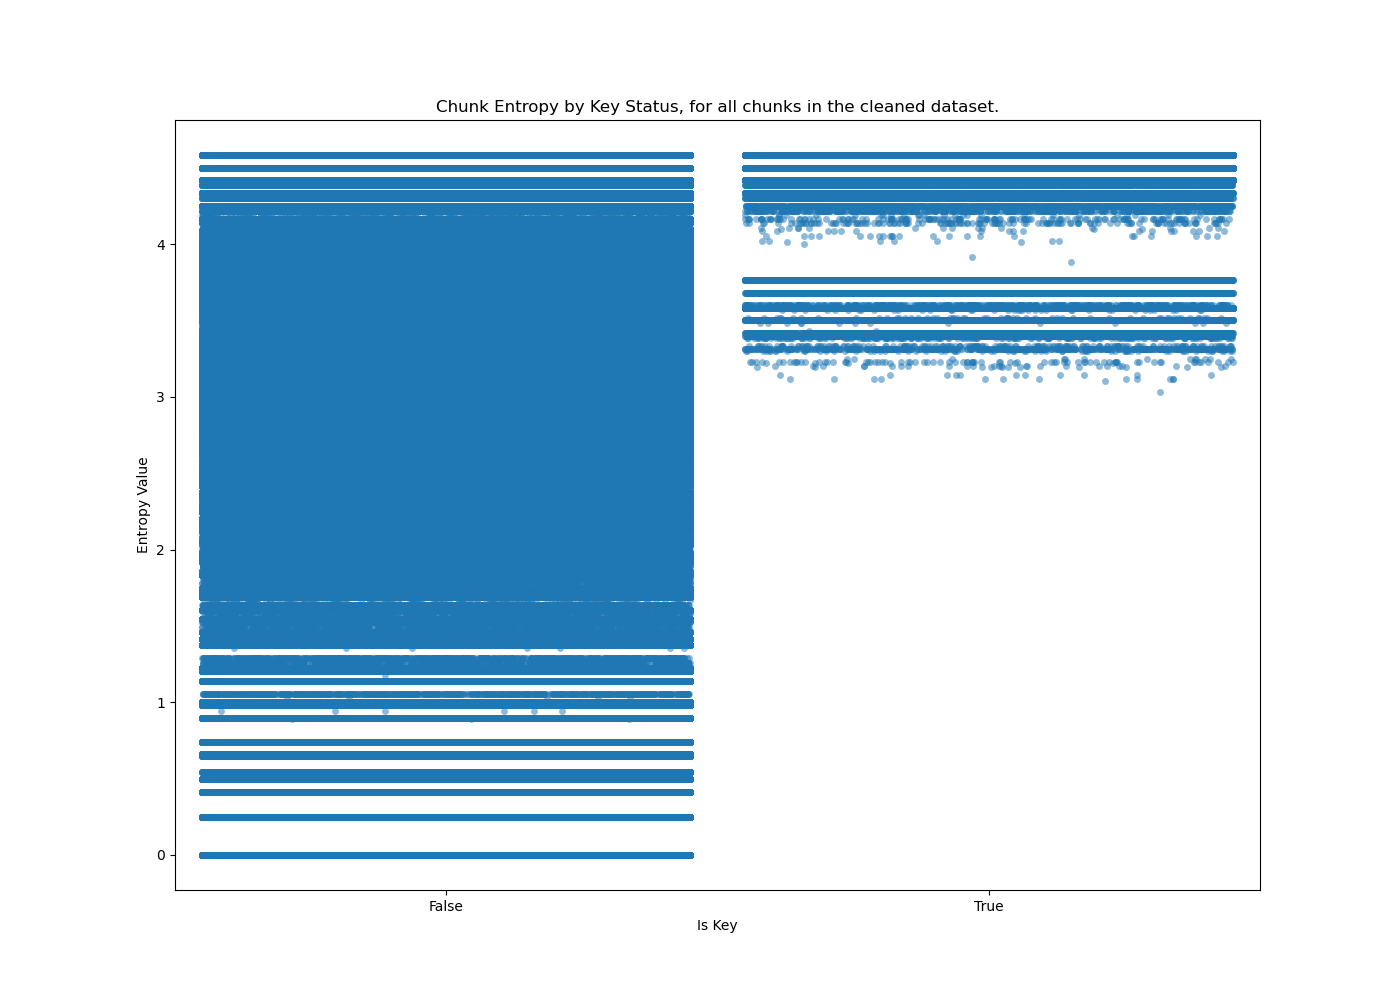
\includegraphics[width=16cm]{plots/chunk_entropy_by_key_status.png}
        \caption{Visualization of the entropy distribution for all chunks of the \textit{phdtrack\_data\_clean/} RAW heap dump dataset.}
    \end{figure}

    Using a script to perform some counting, we realize that the number of chunks whose entropy is less than the minimum entropy of the chunks that contains a key (is key chunk) is 19690826, which represents 52.3\% of the total number of chunks. It's not entirely clear why the key chunk entropy values seem spread across 2 strips of values, but is probably an effect of the different distributions of chunks across the input dataset, depending on the version, use can and number of chunks in the considered input files.

    After all those extensive analysis and tests, we have gained invaluable knowledge about how we can reduce the scale of the problem and parse the files. Now, we need a way to create meaningful embeddings for the blocks we want to perform machine learning on. This is the goal of the next section.

\section{Graph-based memory dumps embedding}\label{chap:mem_2_graph}
Now that we have a decent understanding of the dataset as well as the low level memory dump format, we can start to think about how to convert the memory dumps into graphs. As a recall, we want to be able to convert a memory dump into a graph representation that can be used for machine learning, since we want to be able to create a memory modelization as a basis for efficient embedding and feature engineering later. This is inherently due to the imbalanceness of the dataset, as we want to add more information to each memory block that just its raw bytes. The goal is to have a graph representation of the memory dump that can be used for efficient machine learning.

\subsection{Initial work from Python to Rust}

Initially, we have been working and manipulating the code provided by SmartKex\footnote{SmartKex GitHub repository: \url{https://github.com/smartvmi/Smart-and-Naive-SSH-Key-Extraction}} for key detection. Our first explorations of the dataset quickly gave birth to some Jupyter Notebooks, which were used to explore the dataset and to understand the code, like \texttt{search\_in\_heap\_mem.ipynb}. Rapidly, we decided to rebuild a complete Python 3.11 version of the code. This was done for several reasons:

\begin{itemize}
    \item The provided code had no type hinting, which makes it hard to read and understand.
    \item We wanted to explore the dataset and learn by doing.
    \item The original code was not designed to be used as a library, but rather as a standalone script.
    \item The original code was just a few hundred lines of code and was not designed to be easily extensible, nor to be able to handle a large number of memory dumps.
    \item We wanted to modernize code by using the latest stable version of Python.
\end{itemize}

We decided to build a memory graph representation at that moment because we wanted to be able to add more information to the memory blocks than just their raw bytes. This new program was called \texttt{ssh\_key\_discover}, and relied on a number of Python libraries to work, like \texttt{graphviz}. This was a all-in-one library, composed of 2 sections, \texttt{mem\_graph} and \texttt{ml\_discovery}. The first one was devoted to build memory graphs, while the second one was dedicated to the data science and machine learning part.

This initial program was already capable of handling several data processing pipelines, including machine learning pipelines with models like Random Forest, a grid search for hyperparameter optimization, a cross validation pipeline, several balancing strategies and of course, a memory graph representation with a semantic embedding. As an early development version, this program was not optimized for performance, and just loading a given heap dump file and its annotation, then building the memory graph representation could take from 30 seconds to a minute (on the TUXEDO machine), depending on the size of the heap dump file. As the original dataset comprises more than $ 10^{6} $ files, a rapid estimation of the time needed just for the semantic embedding of the memory graph representation was above a month. In this regard, this initial program was just used on a bunch of files as a way to develop the semantic embedding model, parsing algorithms and start working on feature engineering and machine learning. But it could not be used to produce final results on the whole dataset due to the performance issues described above.

Such an optimization issue was clearly not acceptable, and we decided to rewrite the graph part in Rust. This is a compiled language that leverages zero-cost abstractions, and thus, is several order of magnitude faster than Python. It was also a good opportunity to learn Rust, which is a language that is gaining more and more popularity, especially in the security community. This new program was called \texttt{mem2graph}. Switching from Rust to Python and doing a proper use of multithreading allowed us to reduce the time needed to build the memory graph representation from 30 seconds to less than 1 second. In out case, and comparing using only the TUXEDO laptop, this represents an estimated minimum of a 130x speedup. But this is even much better on the server, where the multithreading can really be leverage. This was a significant improvement which allowed us to build the memory graph representation for the whole original dataset in just a few hours.

\subsection{Memory Graph Representation}
Now, let's describe the memory graph representation. The goal is to be able to represent a memory dump as a graph. This modelization makes sense since the heap dump can be considered as having memory chunks as nodes, being connected by pointers acting as arrows. This is a very natural way to represent a memory dump. However, in our cases, and since the goal is to make predictions on raw bytes, we will not use the chunks as nodes, but rather the memory blocks directly. This is because we want to be able to make predictions on raw blocks of bytes, and not on chunks. 

% introduce the type of the graph, the nodes and edge
Our memory graph representation is composed of a directed graph, where each node is a memory block of bytes, and each edge is either indicative of a pointer link or a chunk membership relationship. This second representation is directly inspired by collection representation in \acrlong{kg} ontologies. In the case of \acrshort{rdf}, this could be equivalent to a \textbf{rdf:Bag}, which is an unordered container \cite{OrderedDataInRDF20} (see \ref{sec:background:ontology}). The graph is directed because the pointers are directed. We will also consider the relationship of belonging to a chunk as oriented from the data structure header block to the data structure member blocks.

Our memory graph representation is inherently a property graph. Each node and edge can have properties. The properties of an edge are the type of the edge, which can be either a pointer or a structure membership relationship.

\begin{itemize}
    \item \textbf{dts:} Data Structure Membership Relationship
    \item \textbf{ptr:} Pointer Relationship (direction is from the source to the target)
\end{itemize}

In our case, the properties of a node are at minimum the address and the byte block. The graph is also heterogeneous since our nodes can have different types corresponding to their inferred characteristics. 

\begin{itemize}
    \item \textbf{PN:} Pointer Node. This is a node whose bytes have been identified as a pointer.
    \item \textbf{CHN:} Chunk Header Node. This is a node whose bytes have been identified as a memory (malloc) chunk header. In the graph, this node is the root node of a memory structure managed by the C library responsible for memory management and allocation.
    \item \textbf{KN:} Key Node. This is a node whose bytes have been identified as a key. This identification relies both on the annotations and some verification checks.
    \item \textbf{VN:} Value Node. These are all blocks that have not been identified. It is the default node type.
\end{itemize}

These nodes and edges form the base of the memory graph representation. Below is a simplified (truncated) example of a memory graph representation. The full example is available in \ref{appendix:mem_graph:17016-1643962152:full}. For clarity, the addresses are not displayed in this simplified version. Another version of this graph with real addresses is available in \ref{appendix:mem_graph:17016-1643962152:truncated}.

\begin{figure}[H]\label{methods:mem_graph:17016-1643962152:simplified}
    \centering
    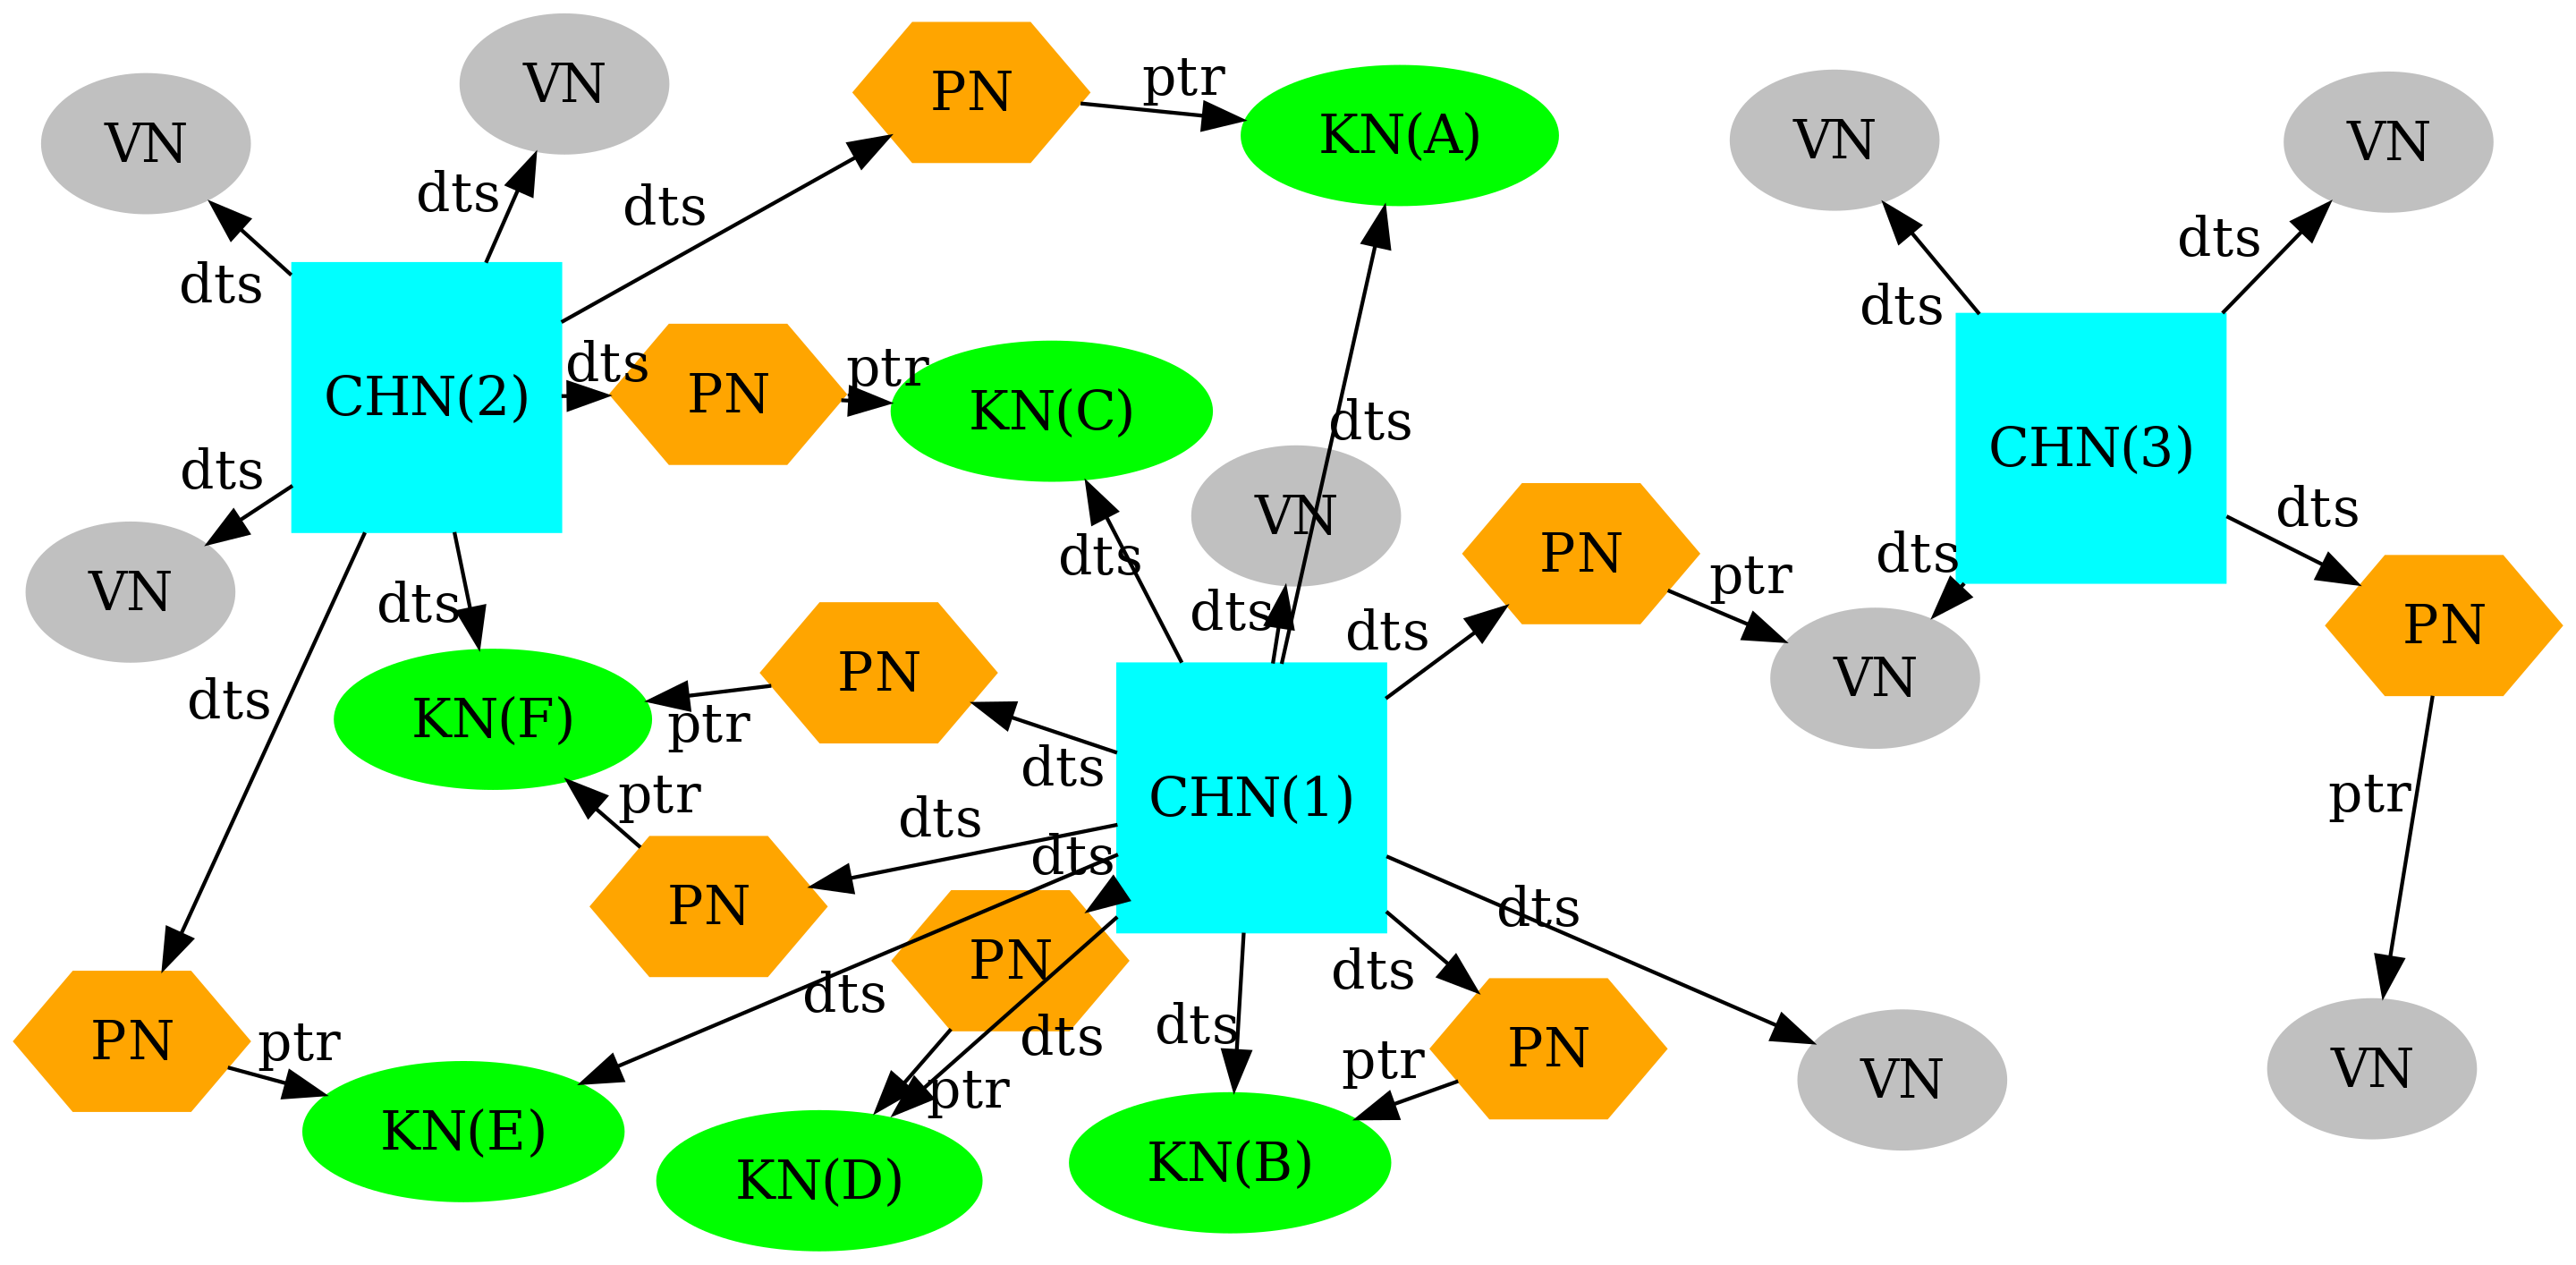
\includegraphics[width=16cm]{graphs/17016-1643962152_truncated_no_addresses_corrected.png}
    \caption{Visualization of a truncated memory graph generated from \textit{Training/basic/V\_7\_1\_P1/24/17016-1643962152-heap.raw}. The addresses are not displayed for improved readability. Version with addresses here \ref{appendix:mem_graph:17016-1643962152:truncated}.}
\end{figure}

The given graph represents a memory layout with various types of nodes, each serving a specific purpose. The graph contains \gls{chn} nodes, which act as the root nodes for allocated structures and are colored in cyan. These DTN nodes are connected to \gls{kn} nodes, which are identified as keys and are colored in green. The \gls{pn} nodes, colored in orange, are pointers and can be connected to value nodes or key nodes. Finally, the graph includes \gls{vn} nodes, which are the default node types and are colored in gray. These nodes have not been identified as any specific type and may contain arbitrary values.

The idea behind this representation will be to try to make predictions on the \gls{kn} nodes, which are the nodes that have been identified as keys. Using the graph, we can build an embedding of the nodes and as such, add more information to a given byte block than just its raw bytes. This is the basis of the semantic embedding, which will be discussed later.

This example is based on the heap dump file \textit{Training/basic/V\_7\_1\_P1/24/17016-1643962152-heap.raw} and has been generated using \texttt{mem2graph}, and the \textbf{sfdp} layout algorithm from \texttt{graphviz} using the following command:

\begin{lstlisting}[language=bash, caption={Command used to generate the memory graph visualization of \textit{Training/basic/V\_7\_1\_P1/24/17016-1643962152-heap.raw}}]
    sfdp -Gsize=30! -Goverlap=voronoi -Tpng 17016-1643962152_truncated_no_addresses.gv > 17016-1643962152_truncated_no_addresses.png
\end{lstlisting}

\section{From heap dump to memory graph embeddings}
Now that the basis of the memory graph representation has been described, let's dive in the different phases involved in transforming a raw heap dump file into a memory graph file with some custom embeddings that can later be loaded and used by some data analysis and \acrshort{ml} programs.

\subsection{Initialization and data checking}

The graph construction process begins with the initialization phase. In this phase, the first step is graph initialization, which involves loading a given heap dump file and its associated annotation file. Once the files are loaded, several checks are performed on the annotation file to ensure its validity. These checks include verifying that all annotations are present and formatted correctly, as well as ensuring that the annotation file is neither empty nor contains errors.

\subsubsection{Graph Construction steps}

The second major step in the process is graph building. This involves constructing the graph from heap dump byte blocks. The first part of this step is the data structure detection, where blocks are parsed from start to finish. The parsing process leaps over blocks by using chunk sizes that are stored in chained chunk headers. Each chunk is then verified for its size, alignment, and the presence of a potential footer. Following this, the pointer detection step is carried out. In this phase, potential pointers are identified using the previously introduced pointer detection algorithm and are added to the graph. 

An optional step that can be performed is the chunk pointer reduction. This step removes any blocks that are not Chunk Header Nodes, effectively transforming the graph from a block-based graph to a chunk-based graph. While this step is not mandatory, it can be useful for reducing the scale of the problem. This approach will be extensively used in the machine learning section, as it has been shown that the key block prediction problem is equivalent to a key chunk prediction problem.

\subsubsection{Graph Annotation}

The third major step in the process is graph annotation. In this phase, Value Nodes in the graph are replaced by Key Nodes, utilizing the annotations provided in the JSON annotation file. Additional annotations, such as SSH\_STRUCT, can also be added at this stage. Following the completion of the annotation step, it becomes possible to export the graph for various purposes. The graph can be exported to file formats like \texttt{.dot} or \texttt{.gv}, which are suitable for visualization or other analytical tasks.

At this step, the graph is looking similar to the example shown before \ref{methods:mem_graph:17016-1643962152:simplified}. Using the pointer reduction to a chunk-only \gls{memgraph}, we can obtain something like the following:

\begin{figure}[H]\label{methods:mem_graph:585-1644391327:chunk_only}
    \centering
    \includegraphics[width=16cm]{graphs/chunk_top_vn_semantic_home_onyr_code_phdtrack_phdtrack_data_clean_585-1644391327-heap.raw_dot_no_vn_chn_annotation_no_vn-sfdp.png}
    \caption{Visualization of the chunk memory graph, with only Chunk Header Nodes representing chunks, generated from \textit{Training/scp/V\_7\_8\_P1/16/
    585-1644391327-heap.raw}.}
\end{figure}

Note how we can identify some data structures formed by pointer-connected chunks. This is a very interesting property of the memory graph representation, since it allows identifying data structures and their members based only on the shape of connections. This is a very important property that will be used later for feature engineering and embeddings. 

\subsubsection{Custom Graph-Based Embeddings}

The fourth step in the workflow involves generating embeddings from the graph. Multiple types of embeddings can be generated, each serving a unique purpose and offering different insights into the graph structure. One such embedding is the semantic embedding. This is a general approach that enriches each node with information related to its graph structure vicinity. It captures the essence of the node's position and relationships within the graph, making it useful for various machine learning and analytics tasks.

In addition to semantic embeddings, other types of embeddings can also be generated. For instance, statistical embeddings focus on capturing the statistical properties of the graph. Another interesting type of embedding is the random walk embedding and related version called Node2Vec. This method leverages the random walk algorithm to generate embeddings, capturing the local and global structure of the graph by simulating random paths through it.

Each of these embeddings offers a unique lens through which to analyze and interpret the graph, and the choice of embedding can be tailored to the specific requirements of the task at hand. It's also possible to add additional features like entropy of the chunk start bytes and filtering information.

\subsubsection{Exporting the Graph}

The fifth step in the process involves exporting the graph. The graph is exported to a \texttt{.gv} DOT file format. Custom embeddings are integrated into the graph by utilizing the comment fields in a slightly modified stringified JSON format. This approach allows for easy reading of the embeddings associated with each node while maintaining the DOT file as a valid format that can be used with tools and libraries supporting the DOT graph formal.

The DOT (Directed Orthogonal Text) format is a plain text graph description language that is widely used for representing structured information. An example of a \gls{memgraph} in DOT format without embeddings is provided for reference. In this example, nodes and edges are represented along with their attributes such as color, shape, and labels.

When embeddings are added to the graph, additional comment fields are included in the DOT file nodes. These comment fields contain a JSON string that holds the embedding information for each node. Moreover, the graph starts with a pseudo JSON comment field that contains a serialized JSON object specifying the embedding type and feature names. 

Here is an example of a comment field in a node:

\begin{lstlisting}[style=text, caption={A comment field example for a node with embedding. Output is cropped.}]
    comment="[0,94918015119368,1,108,108,108,108,108,108,108,1,67,82,139,175,204,...
    0,0,2.355388542207534]"
\end{lstlisting}

Below is an example of a \gls{memgraph} comment field containing a JSON serialized object with embedding type and feature names.

\begin{lstlisting}[style=text, caption={A memgraph comment field example containing JSON serialized object with embedding type and feature names. Output is cropped.}]
    comment="{ 'embedding-type': 'chunk-semantic-embedding', 'embedding-fields': ['block_position_in_chunk','chn_addr','chns_ancestor_1',...'chns_children_8','chunk_byte_size','chunk_number_in_heap','chunk_ptrs','chunk_vns','ptrs_ancestor_1','ptrs_ancestor_2',...,'ptrs_children_8','entropy'] }"
\end{lstlisting}

The inclusion of these comment fields serves multiple purposes. First, it allows for the storage of embeddings along with additional information, making the graph more informative. Second, this format can be easily integrated into Python machine learning pipelines, facilitating the use of the graph in various machine learning tasks. Lastly, the DOT format serves as a standard format for graph representation, making it a versatile choice for both visualization and computational tasks.

\section{A wide range of features and embeddings}
In the following, we will explore the features and embeddings developed and used in this thesis. We will start by the features and embeddings based on the memory graph characteristics, then we will explore the graph-agnostic embeddings, and finally, we will discuss the machine learning models used for the binary classification task.

\subsection{Embeddings based on custom features}
While doing the construction of the graph, we can add some custom features to the nodes. Those features have been developed to embed the unique characteristics of each node of the graph, depending on its type, parent chunk characteristics as well as its vicinity in the memory graph. Those features have been regrouped in several custom embeddings that will be discussed in the following.

\subsubsection{Remark on the collaborative work}
This section focuses on the embeddings developed during a Masterarbeit project around OpenSSH heap dump analysis. Clément Lahoche and the author of the present report have done a collaborative effort on the matter. Since Clément has focused on the embeddings, the following section will not discuss in too many details the embeddings that are already described and analyzed in details by Clément's work. The reader is invited to read his Masterarbeit report \cite{ClementEmbeddingsMasterarbeit23} for more information. This section includes some elements that are clearly identified as coming from Clément's work.

As a notable difference, the Node2Vec embedding, which is a graph-agnostic embedding, will also be discussed in the following, which is not the case in Clément's thesis. This is because the present report focuses on the machine learning part, and especially on graph representation learning.

\subsubsection{Semantic graph embedding}\label{sec:mem_2_graph:semantic_embedding}

The focus of this stage is on semantic embedding, a technique that transforms the graph into a low-dimensional vector space. Each vector encapsulates the local neighborhood of a graph chunk, enabling the application of advanced machine learning methods. The embedding process is intricate, considering both direct and indirect connections to and from each chunk. It starts by counting the number of pointers and chunks directly linked to a specific chunk, and then extends this by recursively exploring deeper layers of connections. A parallel reverse analysis is also conducted to capture child nodes. The outcome is a compact vector that richly represents the chunk's contextual relationships within the graph.

The following algorithm describes the process of generating the semantic embedding for a given chunk:

\begin{algorithm}[H]
    \caption{Generate Ancestor/Children Embedding.}
    \label{algo:embedding:generate_ancestor_children_embedding}
    \begin{algorithmic}
        \Function{GenerateNeighborsCHN}{$chunk\_node, dir$}
            \State $ancestor\_nodes \gets$ an empty set
            \State $children \gets$ graph.neighbors\_directed($chunk\_node, OUT$) \Comment{Get members of the chunk}
            \For{$child$ \textbf{in} $children$}
                \State $ancestor\_nodes$.insert($child$)
            \EndFor
            \State $result \gets$ an empty list
            \State $current\_nodes \gets$ an empty set
            \For{$\_$ \textbf{in} $0$ \textbf{to} $DEPTH$}
                \State $current\_nodes \gets$ $ancestor\_nodes$ \Comment{switch ancestor nodes and current nodes}
                \State $ancestor\_nodes \gets$ an empty set
                \State $nb\_chn \gets 0$
                \State $nb\_ptr \gets 0$
                \For{$current\_node$ \textbf{in} $current\_nodes$}
                    \If{$node$ is ChunkHeaderNode} \Comment{Update number of chunks and pointers}
                        \State $nb\_chn \gets nb\_dtn + 1$
                    \ElsIf{$node$ is PointerNode}
                        \State $nb\_ptr \gets nb\_ptr + 1$
                    \EndIf
                    \Comment{Get neighbors of the current node}
                    \For{$neighbor$ \textbf{in} graph.neighbors\_directed($current\_node, dir$)}
                        \State $ancestor\_nodes$.insert($neighbor$) \Comment{Add neighbors to the next ancestor nodes}
                    \EndFor
                \EndFor
                \State $result$.append($nb\_chn$) \Comment{Add number of data structures}
                \State $result$.append($nb\_ptr$) \Comment{Add number of pointers}
            \EndFor
            \State \textbf{return} $result$
        \EndFunction
    \end{algorithmic}
\end{algorithm}

Note that this algorithm is taken from \citeauthor{ClementEmbeddingsMasterarbeit23}, from his Masterarbeit report \cite{ClementEmbeddingsMasterarbeit23}. It has been developed and implemented as a collaborative effort on this project.

The embedding algorithm is applied to each chunk in the graph, exploring up to a predefined depth, generally 8, which is a hyperparameter of this embedding. This results in a 32-unit embedding, broken down into 8 units each for ancestor pointers, ancestor chunks, child pointers, and child chunks. Basic chunk attributes like block position, byte size, and number of pointers and value nodes are also included, bringing the total embedding size to 37 units. Despite its comprehensiveness, the embedding has limitations, such as the potential for noise from value nodes and the complexity of capturing intricate relationships.

A way that have been used extensively, to both reduce the number of nodes and to improve the quality of the embeddings, is to reduce the graph to a chunk-only graph. This is done by removing all the nodes that are not chunk header nodes. It is a very interesting approach, since it allows to reduce the scale of the problem by a factor of 10, and also allows focusing on the data structures, which are the most interesting nodes to embed. This approach will be used in the machine learning section, since we have shifted the focus from block to chunk prediction.

\subsubsection{Semantic features from essential chunks attributes}

Every chunk in the heap dump comes with fundamental attributes that provide insights on its structure and content. These attributes are not limited to the primary chunk nodes but are also inherited by value and pointer nodes, which are subcomponents of a chunk. The key attributes include the block's position within the chunk, the chunk's byte size, the total number of pointers and value nodes in the chunk, and the chunk's index in the heap. These details collectively offer a thorough understanding of each chunk's makeup and its relative position in the heap.

\subsubsection{Statistical Embedding}

Statistical embeddings serve as a powerful tool for reducing high-dimensional data while preserving essential patterns and probabilistic relationships. One key technique employed is the use of n-gram values, specifically focusing on bit combinations to manage dimensionality. This approach aligns with the primary goal of identifying SSH keys, which inherently display a wide range of frequencies. Various n-gram sizes are utilized, including 1-gram, 2-gram, 3-gram, up to 8-gram, with the latter contributing significantly to capturing broader contextual patterns. 

In addition to n-grams, other statistical metrics like mean, standard deviation, MAD, skewness, kurtosis, and Shannon entropy are incorporated. These metrics offer a multi-faceted view of the data, aiding in the identification of SSH keys. However, chunks with a standard deviation of zero are excluded from the analysis, as they are unlikely to contribute to the identification of random patterns like SSH keys. These skipped values are replaced with \texttt{NaN} values in embedding comment of nodes, that needs to be handled by the machine learning pipeline. It has been chosen to replace those values with zeros. 

Finally, the statistical embedding vector for each chunk is constructed by combining n-gram values and these additional statistical metrics. The vector also includes basic chunk information, resulting in a comprehensive vector that encapsulates the chunk's characteristics.

\subsubsection{Start-bytes Embedding}
In addition to the aforementioned embeddings, a simpler approach was implemented to serve as a baseline for comparison. This method focuses solely on the initial bytes of each chunk for vectorization. The sample vector is initialized with basic chunk information and then populated with the first bytes of the chunk, up to a predefined limit. If the chunk has fewer starting bytes than the predefined limit, zeros are added to fill the remaining positions. This straightforward approach provides a straightforward embedding, suitable for comparative evaluations with more intricate embeddings.

\subsection{Embedding transformations depending on the model}

When it comes to feeding embeddings into machine learning models, the shape and size of the embeddings need to be tailored to fit the model's requirements. For classic machine learning algorithms like Random Forest, the requirement is that the embedding matrices must be of a fixed, predefined size. This presents a unique challenge when working with graph embeddings, as graphs usually have a variable number of nodes. To address this, padding is added to the embedding matrices to ensure they all match the size of the largest graph. In contrast, Graph Convolutional Networks (GCN) offer more flexibility in this aspect. GCNs are capable of handling variable-size embedding matrices as long as the number of features is fixed. This eliminates the need for padding the matrices, which is advantageous as it simplifies the preprocessing steps.

\subsubsection{Node filtering to feature}

On the topic of node filtering in the context of chunk memory graphs, it's important to note that active rebalancing isn't performed, despite the number of positive nodes (key chunks) being substantially lower than the number of negative nodes (non-key chunks). The rationale behind this choice is to enable models to learn from complete graphs. This is particularly relevant for Graph Convolutional Networks, which are capable of handling graphs of variable sizes. The goal is for the models to be able to identify key chunks even in completely unlabeled memory graphs. The ability of GCNs to process variable-size graphs makes them especially suitable for this kind of task, as it allows the model to learn from the full structure of the graph without the need for compromising the integrity of the data through techniques like rebalancing.

\subsection{Graph-agnostic Embeddings}

Unlike our previous embeddings, which were developed manually to suit the intricacies of chunk graphs, there are also pre-existing, generalized graph embeddings. These graph-agnostic embeddings offer the benefit of being applicable to a wide range of graphs without requiring specific customization based on the characteristics of the underlying data.

\subsubsection{RandomWalk}

The RandomWalk algorithm offers a straightforward approach to graph embedding. It simulates random walks starting from each node in the graph and uses these walks to create vector representations of the nodes. One of the advantages of RandomWalk is its simplicity, both in terms of implementation and interpretation. The algorithm excels at capturing local structures within the graph, making it particularly effective for tasks such as community detection and link prediction. However, its focus on local characteristics means that it might not capture global properties of the graph as effectively.

\subsubsection{Node2Vec}

Node2Vec extends the capabilities of the RandomWalk algorithm by introducing additional parameters that allow for a more nuanced exploration of the graph. This makes Node2Vec more versatile than RandomWalk, enabling it to capture both local and global graph structures. Because of its flexibility, Node2Vec is well-suited for a range of applications including the specific task of providing an embedding for the node of memory graphs. While its versatility is a strong point, it comes at the cost of increased computational complexity due to the introduction of several hyperparameters.

\textbf{Hyperparameters:}
\begin{itemize}
  \item \textbf{p:} The return parameter, which controls the likelihood of the walk returning to the node it just left.
  \item \textbf{q:} The in-out parameter, which differentiates between inward and outward nodes in the walk.
  \item \textbf{Length of Walk:} Determines the length of each random walk.
  \item \textbf{Number of Walks:} Specifies the number of walks to initiate from each node.
\end{itemize}

Note that the two last hyperparameters have a huge impact on the performance of the algorithm. These hyperparameters play a crucial role in shaping the behavior of the Node2Vec algorithm. Specifically, the return and in-out parameters help guide the random walks in a way that allows the algorithm to capture different types of structural information from the graph. The length and number of walks, meanwhile, impact the granularity and quality of the embeddings generated.

\section{Machine Learning Binary Classification}

Binary classification is a type of machine learning task where the model is trained to differentiate between two classes. In the context of key chunk prediction, binary classification serves to identify whether a given chunk is a "key chunk" or not. Successfully predicting key chunks is crucial as it leads to a 100\% successful key retrieval rate. This is because, in our case, all keys are situated at the beginning of a chunk, and no chunk contains more than one key. Various machine learning models, ranging from classic approaches to more modern methods like Graph Convolutional Networks (GCNs), have been employed for this task.

\subsection{Classic Models of Machine Learning}

For baseline comparisons, we have experimented with classic machine learning models including Random Forest, Logistic Regression, and the SGD Classifier. These models serve as a well-studied and understood starting point for our classification problem, providing a frame of reference against which more complex models can be compared.

\subsubsection{Random Forest}

Random Forest is an ensemble learning method that operates by constructing multiple decision trees during training and outputs the class that is the mode of the classes of the individual trees for classification tasks. It is highly flexible and can handle a wide range of data types, making it a strong candidate for various use cases, including key chunk prediction.

\textbf{Strong and Weak Points:}
\begin{itemize}
  \item \textbf{Strong:} The model is robust to overfitting and can handle high dimensional data well.
  \item \textbf{Weak:} Random Forest models can be computationally expensive and may require a long training time, especially for larger datasets.
\end{itemize}

As often with models, Random Forest has a bunch of hyperparameters:

\textbf{Hyperparameters:}
\begin{itemize}
  \item \textbf{n\_estimators:} Number of trees in the forest.
  \item \textbf{max\_features:} The number of features to consider when looking for the best split.
  \item \textbf{max\_depth:} The maximum depth of the tree.
  \item \textbf{min\_samples\_split:} The minimum number of samples required to split an internal node.
  \item \textbf{min\_samples\_leaf:} The minimum number of samples required to be at a leaf node.
\end{itemize}

We have used the implementation of Random Forest available in the Scikit-learn library \cite{ScikitLearn}.

\subsubsection{Logistic Regression}

Logistic Regression is a statistical model commonly used for binary classification tasks. It models the log-odds of the probability of the event occurring as a linear combination of the predictor variables. The model is particularly effective when the probability of the outcome (dependent variable) can be expressed as a logistic function of the predictor (independent variable).

\textbf{Strong and Weak Points:}
Logistic Regression is straightforward to implement and understand, making it a good starting point for many classification problems. However, its simplicity is both a strength and a weakness; it might not perform well when the relationship between the variables is not log-linear or when the dataset has high dimensionality.

\textbf{Hyperparameters:}
\begin{itemize}
  \item \textbf{C:} Inverse of regularization strength; smaller values specify stronger regularization.
  \item \textbf{solver:} Algorithm to use for optimization, such as 'liblinear' or 'saga'.
  \item \textbf{max\_iter:} Maximum number of iterations for the solver to converge.
\end{itemize}

We have relied on the Logistic Regression implementation available in the Scikit-learn library for our experiments\cite{ScikitLearn}, using the default hyperparameters.

\subsubsection{SGD Classifier}

The Stochastic Gradient Descent (SGD) Classifier is a linear classifier optimized by stochastic gradient descent. It is especially useful for large-scale and sparse machine learning problems. The SGD Classifier can approximate other types of linear classifiers like Logistic Regression and Support Vector Machines.

\textbf{Strong and Weak Points:}
SGD Classifier is computationally efficient, making it well-suited for large datasets. However, it requires careful tuning of its hyperparameters and might be sensitive to feature scaling.

\textbf{Hyperparameters:}
\begin{itemize}
  \item \textbf{alpha:} Regularization term that discourages large coefficients to prevent overfitting.
  \item \textbf{loss:} Specifies the loss function to be used, such as 'hinge' for SVM or 'log' for logistic regression.
  \item \textbf{max\_iter:} Maximum number of passes over the training data.
  \item \textbf{learning\_rate:} The learning rate schedule, could be 'constant', 'optimal', 'invscaling', or 'adaptive'.
\end{itemize}

For the SGD Classifier as well, we used the Scikit-learn implementation\cite{ScikitLearn}.

\subsection{Graph Convolutional Networks (GCN)}

As GCNs have already been introduced in the background section, this part will primarily focus on our specific implementation and the variants of GCN models employed for the task of key chunk prediction.

GCNs are a specialized form of neural networks designed to operate directly on graphs. One of their main characteristics is their ability to capture the graph's structural information. They accomplish this by using edge connectivity information, either from an adjacency matrix or an edge list, as part of their input. This makes them particularly effective for tasks involving irregular data structures like the memory graphs discussed previously.

We used the PyTorch Geometric library for the development of our GCN models. This library offers a robust set of tools and abstractions, making it easier to construct custom graph-based neural networks \cite{PyTorchGeometric19}.

GCNs excel at capturing the topological features of graphs, making them a strong candidate for our task of key chunk prediction. However, they can be computationally intensive, especially for large graphs, and also require careful tuning of hyperparameters for optimal performance.

\subsubsection{Very Simple GCN}

The Very Simple GCN model is a minimalist approach, capturing the essential features of a Graph Convolutional Network. This model consists of just one graph convolution layer followed by a single fully connected layer. The convolution layer takes the input features and transforms them into a 16-dimensional space.

After the graph convolution operation, a ReLU (Rectified Linear Unit) activation function is applied to the output. ReLU is defined as \( f(x) = \max(0, x) \), replacing all negative values in the tensor with zeros. In the context of GCNs, ReLU is commonly used to introduce non-linearity into the model. It enables the network to learn from the error and make adjustments, making it more capable of handling complex, non-linear relationships in the graph data.

Finally, the output from the ReLU activation is passed through a fully connected layer to produce the final output for classification. Due to its simplicity, this model is computationally efficient but may not capture complex graph structures effectively.

\subsubsection{Simple GCN Models}

The Simple GCN model, or \texttt{LessSimplifiedGNN}, is a step-up in complexity from the very simplified version. It incorporates two graph convolutional layers, doubling the depth of the network. The first convolution transforms the input features to a 12-dimensional space, and the second one further transforms these 12-dimensional vectors into 24 dimensions. Two fully connected layers follow, ultimately producing the final output. This model is capable of capturing more complex features in the graph but is computationally more demanding than the simpler model.

\subsubsection{First GCN Model}

The First GCN model is the first version that was actually implemented and tested for the task. It's a more complex architecture optimized for higher performance. It consists of two graph convolution layers that transform the input features first into a 16-dimensional and then into a 32-dimensional space. Following these, the network contains three fully connected layers. These layers are intended to capture more intricate patterns in the data. Failed attempts to scale the model computation speed by delegating the fully connected layers to the GPU were made, but ultimately, the model was too memory intensive to be trained on the GPU. This model is designed for capturing more nuanced relationships in the graph but at the cost of higher computational requirements.

\subsection{The Impact of Complexity}

The complexity of a model is a double-edged sword when it comes to performance metrics like precision and recall. On one hand, more complex models with additional layers or more neurons can capture intricate patterns in the graph data, potentially improving precision by accurately identifying key chunks. On the other hand, the complexity often leads to overfitting, especially when the training dataset is small or lacks diversity. Overfitting can adversely affect recall, as the model might become too specialized in recognizing training graphs and fail to generalize well to unseen data.

In the case of Graph Convolutional Networks (GCNs), the non-linear transformations and multiple layers can allow the network to learn highly specialized features, which is excellent for achieving high precision. However, these can be detrimental to recall if the model becomes so tailored to the training data that it fails to identify key chunks in new, unseen graphs.

The impact of the model's complexity also varies with the number of input graphs. For datasets with few graphs, a simpler model is often more appropriate to prevent overfitting. In contrast, when numerous diverse graphs are available for training, a more complex model can be employed to capture the rich set of features inherent in the data, thereby potentially improving both precision and recall.

Therefore, the choice of model complexity should be carefully considered, weighing its impact on performance metrics and the size and diversity of the available training data. This is why more complex GCN models have also been implemented and tested.

\subsection{Understanding Dropout in GCNs}

Dropout is a regularization technique used in neural networks, including Graph Convolutional Networks (GCNs) and Convolutional Neural Networks (CNNs), to prevent overfitting. The dropout layer randomly sets a fraction of the input units to 0 during training, which helps to make the model more robust and improves generalization. In the \acrshort{ml} pipelines developed in Python, a dropout rate of 0.5 is used, meaning approximately 50\% of the neurons will be turned off during each forward pass. This section will discuss the effect of dropout on the model's performance and the intuition behind it.

\subsubsection{Effect on Binary Classification}

In a binary classification problem, dropout can have several effects:

\begin{itemize}
    \item \textbf{Reduced Overfitting}: By randomly deactivating neurons, the model is less likely to rely on any single feature, making it generalize better to unseen data. This is expected to reduce overfitting and thus improve the model's performance, especially the recall of the positive class.
    \item \textbf{Increased Robustness}: Dropout can make the model more robust to noise in the training data.
    \item \textbf{Variable Performance}: While dropout can improve generalization, it may also lead to increased variance in the model's predictions, especially if the dropout rate is too high.
\end{itemize}

In the code of some GCN models implemented, dropout is applied after the activation functions of the GCN layers and the first fully connected layer:

\begin{verbatim}
    x = F.relu(x)
    x = self.dropout(x)
\end{verbatim}

This is a common practice as it allows the model to learn more robust features. However, the dropout rate and its placement in the architecture are yet other hyperparameters that may need to be tuned for optimal performance. Since we already have a large number of hyperparameters, we will not tune the dropout rate in this thesis.

\subsubsection{Batch Normalization}

The code also includes Batch Normalization layers, denoted by \texttt{self.bn1} and \texttt{self.bn2}. These layers normalize the features to have zero mean and unit variance, which can accelerate training and provide some regularization effect, complementing the dropout layers.

\subsection{More Complex GCN Models}

In an effort to enhance the performance of our initial GCN models, we explored more complex architectures. The motivation behind increasing the complexity was to evaluate whether additional layers or techniques could lead to improved performance metrics such as precision and recall. These advanced models have been tested against the simpler GCN models to determine their effectiveness.

\subsubsection{GCN with Dropout and Batch Normalization}

Building upon the First GCN model, we incorporated dropout and batch normalization layers. Dropout is employed to mitigate the issue of overfitting, especially relevant for complex models trained on limited data. With a dropout rate of 0.5 after each ReLU activation, we were able to regulate the model's complexity during training. 

Batch normalization, on the other hand, aims to accelerate training and stabilize the learning process. By normalizing the output features of each layer, batch normalization helps in alleviating internal covariance shift, making the model training more resilient to the choice of hyperparameters.

This version of the model aligns closely with the First GCN model, but the addition of dropout and batch normalization layers offer greater robustness, especially when training on imbalanced or smaller datasets.

\subsubsection{Advanced GCN}

The Advanced GCN model represents the most intricate architecture we have experimented with. This model introduces several additional components compared to the simpler models.

The Advanced GCN consists of three Graph Convolution layers, followed by Batch Normalization layers. The initial Graph Convolution layer transforms the input features into a 32-dimensional space, which is then normalized using \texttt{BatchNorm1d}. The second and third Graph Convolution layers further increase the dimensions to 64 and 128, respectively, also followed by batch normalization steps. These layers aim to capture more complex features from the graph structure.

ReLU (Rectified Linear Unit) activation functions are applied after each batch normalization, introducing non-linearity to the model and helping to capture intricate relationships in the data. Additionally, dropout layers with a rate of 0.5 are placed after each ReLU activation to mitigate the risk of overfitting.

After the Graph Convolution layers, the architecture includes a series of fully connected layers that transform the 128-dimensional feature vector into a 256-dimensional space, which is further compressed into 128 and then 64 dimensions. Finally, the model outputs a vector of dimensions corresponding to the number of classes. Each of these fully connected layers is followed by ReLU activations, except for the final output layer.

\begin{itemize}
    \item \textbf{Graph Conv Layers}: Three layers with dimensions 32, 64, and 128
    \item \textbf{Batch Normalization}: Applied after each Graph Conv layer
    \item \textbf{Fully Connected Layers}: Layers with dimensions 256, 128, and 64
    \item \textbf{Dropout}: Applied after each ReLU activation with a rate of 0.5
\end{itemize}

In summary, the model is engineered to capture more complex relationships in the data, at the cost of increased computational requirements and a higher risk of overfitting, especially when trained on small or less diverse datasets. The dropout and batch normalization layers are integrated to combat overfitting to some extent.

The current chapter has been an overview of the dataset, development environment, and tools used for this thesis. In the next chapter, we will dive deeper into developed programs, experimentations conducted and subsequent results.

